% Template for the submission to:
%   The Annals of Probability           [aop]
%   The Annals of Applied Probability   [aap]
%   The Annals of Statistics            [aos] 
%   The Annals of Applied Statistics    [aoas]
%   Stochastic Systems                  [ssy]
%
%Author: In this template, the places where you need to add information
%        (or delete line) are indicated by {???}.  Mostly the information
%        required is obvious, but some explanations are given in lines starting
%Author:
%All other lines should be ignored.  After editing, there should be
%no instances of ??? after this line.

% use option [preprint] to remove info line at bottom
% journal options: aop,aap,aos,aoas,ssy
% natbib option: authoryear
\documentclass[aoas]{imsart}

\newcommand{\ba}{ {\boldsymbol a} }
\newcommand{\bA}{ {\boldsymbol A} }
\newcommand{\bb}{ {\boldsymbol b} }
\newcommand{\bB}{ {\boldsymbol B} }
\newcommand{\bc}{ {\boldsymbol c} }
\newcommand{\bC}{ {\boldsymbol C} }
\newcommand{\bd}{ {\boldsymbol d} }
\newcommand{\bD}{ {\boldsymbol D} }
\newcommand{\be}{ {\boldsymbol e} }
\newcommand{\bE}{ {\boldsymbol E} }
\newcommand{\boldf}{ {\boldsymbol f} }
\newcommand{\bF}{ {\boldsymbol F} }
\newcommand{\bg}{ {\boldsymbol g} }
\newcommand{\bG}{ {\boldsymbol G} }
\newcommand{\bh}{ {\boldsymbol h} }
\newcommand{\bH}{ {\boldsymbol H} }
\newcommand{\bi}{ {\boldsymbol i} }
\newcommand{\bI}{ {\boldsymbol I} }
\newcommand{\bj}{ {\boldsymbol j} }
\newcommand{\bJ}{ {\boldsymbol J} }
\newcommand{\bk}{ {\boldsymbol k} }
\newcommand{\bK}{ {\boldsymbol K} }
\newcommand{\bl}{ {\boldsymbol l} }
\newcommand{\bL}{ {\boldsymbol L} }
\newcommand{\bm}{ {\boldsymbol m} }
\newcommand{\bM}{ {\boldsymbol M} }
\newcommand{\bn}{ {\boldsymbol n} }
\newcommand{\bN}{ {\boldsymbol N} }
\newcommand{\bo}{ {\boldsymbol o} }
\newcommand{\bO}{ {\boldsymbol O} }
\newcommand{\bp}{ {\boldsymbol p} }
\newcommand{\bP}{ {\boldsymbol P} }
\newcommand{\bq}{ {\boldsymbol q} }
\newcommand{\bQ}{ {\boldsymbol Q} }
\newcommand{\br}{ {\boldsymbol r} }
\newcommand{\bR}{ {\boldsymbol R} }
\newcommand{\bs}{ {\boldsymbol s} }
\newcommand{\bS}{ {\boldsymbol S} }
\newcommand{\bt}{ {\boldsymbol t} }
\newcommand{\bT}{ {\boldsymbol T} }
\newcommand{\bu}{ {\boldsymbol u} }
\newcommand{\bU}{ {\boldsymbol U} }
\newcommand{\bv}{ {\boldsymbol v} }
\newcommand{\bV}{ {\boldsymbol V} }
\newcommand{\bw}{ {\boldsymbol w} }
\newcommand{\bW}{ {\boldsymbol W} }
\newcommand{\bx}{ {\boldsymbol x} }
\newcommand{\bX}{ {\boldsymbol X} }
\newcommand{\by}{ {\boldsymbol y} }
\newcommand{\bY}{ {\boldsymbol Y} }
\newcommand{\bz}{ {\boldsymbol z} }
\newcommand{\bZ}{ {\boldsymbol Z} }
\newcommand{\vc}[1]{\mbox{\boldmath $#1$}}
\newcommand{\balph}{ {\boldsymbol \alpha} }
\newcommand{\balpha}{ {\boldsymbol \alpha} }
\newcommand{\bbet}{ {\boldsymbol \beta} }
\newcommand{\bbeta}{ {\boldsymbol \beta} }
\newcommand{\bgam}{ {\boldsymbol \gamma} }
\newcommand{\bgamma}{ {\boldsymbol \gamma} }
\newcommand{\bGamma}{ {\boldsymbol \Gamma} }
\newcommand{\bdelta}{ {\boldsymbol \delta} }
\newcommand{\bDelta}{ {\boldsymbol \Delta} }
\newcommand{\beps}{ {\boldsymbol \epsilon} }
\newcommand{\bepsilon}{ {\boldsymbol \epsilon} }
\newcommand{\bphi}{ {\boldsymbol \phi} }
\newcommand{\bPhi}{ {\boldsymbol \Phi} }
\newcommand{\bpi}{ {\boldsymbol \pi} }
\newcommand{\bpsi}{ {\boldsymbol \psi} }
\newcommand{\bkap}{ {\boldsymbol \kappa} }
\newcommand{\bkappa}{ {\boldsymbol \kappa} }
\newcommand{\bKappa}{ {\boldsymbol \Kappa} }
\newcommand{\blam}{ {\boldsymbol \lambda} }
\newcommand{\blambda}{ {\boldsymbol \lambda} }
\newcommand{\bLambda}{ {\boldsymbol \Lambda} }
\newcommand{\bmu}{ {\boldsymbol \mu} }
\newcommand{\bMu}{ {\boldsymbol \Mu} }
\newcommand{\bet}{ {\boldsymbol \eta} }
\newcommand{\bome}{ {\boldsymbol \omega} }
\newcommand{\bomega}{ {\boldsymbol \omega} }
\newcommand{\bOmega}{ {\boldsymbol \Omega} }
\newcommand{\bnabla}{ {\boldsymbol \nabla} }
\newcommand{\brho}{ {\boldsymbol \rho} }
\newcommand{\bsigma}{ {\boldsymbol \sigma} }
\newcommand{\bSig}{ {\boldsymbol \Sigma} }
\newcommand{\bSigma}{ {\boldsymbol \Sigma} }
\newcommand{\btheta}{ {\boldsymbol \theta} }
\newcommand{\bTheta}{ {\boldsymbol \Theta} }
\newcommand{\bzeta}{ {\boldsymbol \zeta} }
\newcommand{\bPsi}{ {\boldsymbol \Psi} }
\newcommand{\btau}{ {\boldsymbol \tau} }
\newcommand{\bxi}{ {\boldsymbol \xi} }
\newcommand{\bzero}{ {\boldsymbol 0} }
\newcommand{\bones}{ {\boldsymbol 1} }
\newcommand{\given}{\,|\,}
\newcommand{\sS}{{\cal S}}
\newcommand{\Ss}{{\cal S}}
\newcommand{\Field}{{\cal F}}
\newcommand{\colsp}{{\cal C}}
\newcommand{\nullsp}{{\cal N}}
\newcommand{\rowsp}{{\cal R}}
\newcommand{\tildeC}{\tilde{C}}
\newcommand{\tildeK}{\tilde{K}}
\newcommand{\tildew}{\tilde{w}}
\newcommand{\tildebw}{\tilde{\bw}}
\newcommand{\tildebW}{\tilde{\bW}}
\newcommand{\calC}{{\cal C}}
\newcommand{\calcbC}{{\bf {\cal C}}}

% Do not remove even for final version
\newcommand{\kcomment}[1]{{\color{blue}{\{KR: #1\}}}}
\newcommand{\kc}{\kcomment}


\usepackage{amsmath}
\usepackage{pstricks,pst-grad}
\usepackage{graphicx}
\usepackage{floatrow}
\usepackage[linesnumbered,ruled,vlined]{algorithm2e}
\floatsetup[table]{capposition=top}
% \usepackage{subfig}
\usepackage{subfigure}
\usepackage[utf8]{inputenc}

\usepackage[tableposition = top]{caption} % captions
\usepackage{booktabs}                     % horizontal lines in tables

% == Enable text degree
\usepackage{textcomp}

\usepackage{amsthm,amsmath,natbib}
\RequirePackage[colorlinks,citecolor=blue,urlcolor=blue]{hyperref}

% provide arXiv number if available:
%\arxiv{arXiv:0000.0000}

% == Trygve Test
\usepackage{color, colortbl}
\definecolor{Gray}{gray}{0.9}



% put your definitions there:
\startlocaldefs
\endlocaldefs

\begin{document}

\begin{frontmatter}

% "Title of the paper"
\title{Informative Oceanographic Sampling using Excursion Probabilities for Multivariate Random Fields}
\runtitle{Excursion Probabilities for Informative Sampling}

% indicate corresponding author with \corref{}
% \author{\fnms{John} \snm{Smith}\corref{}\ead[label=e1]{smith@foo.com}\thanksref{t1}}
% \thankstext{t1}{Thanks to somebody} 
% \address{line 1\\ line 2\\ printead{e1}}
% \affiliation{Some University}

\author{\fnms{Trygve Olav} \snm{Fossum}\ead[label=e1]{trygve.o.fossum@ntnu.no}, \fnms{Jo} \snm{Eidsvik}\ead[label=e2]{jo.eidsvik@math.ntnu.no}, \fnms{David} \snm{Ginsbourger} \ead[label=e3]{david.ginsbourger@idiap.ch}  \and \fnms{Kanna} \snm{Rajan}\ead[label=e4]{kanna.rajan@ntnu.no}}

\address{Department of Marine Technology\\ Trondheim, Norway\printead{e1}}
\affiliation{Department of Marine Technology, The Norwegian University of Science and Technology (NTNU), Trondheim, Norway}

\address{Department of Mathematical Sciences \printead{e2}}
\affiliation{Department of Mathematical Sciences, NTNU}

\address{Idiap \printead{e3}}
\affiliation{Uncertainty Quantification and Optimal Design group , Idiap Research Institute, Martigny, Switzerland}

\address{Department of Engineering Cybernetics,\printead{e4}}
\affiliation{Department of Engineering Cybernetics, NTNU}

\runauthor{Fossum et al.}

\begin{abstract}
  We examine experiment design for informative sampling for
  characterizing oceanographic phenomena. Methods are developed
  for efficient spatial sampling using autonomous robotic platforms,
  where the goal is to map the regions of cold and fresh water near a
  river mouth. Specifically, we define a design criterion based on
  reducing uncertainty of excursion sets in the context of multivariate
  random fields. We develop analytical expressions for the expected
  variance reduction in excursion sets, and show how these can be
  applicable for static designs and sequential designs building on
  myopic and look-ahead planning. We use simulations to study the
  properties of the suggested methods. Results from field
  deployments with an autonomous underwater vehicle are also presented.

%Motivated by the challenges related to efficient allocation of sampling resources in environmental sensing, the combination of Excursion Probabilities and Gaussian process modeling is explored for autonomous robotic sampling of ocean features; enabling information driven measures  sampling efforts to high-interest regions. These regions are usually characterized by gradients of measurable environmental variables, e.g., temperature or salinity gradients, on which EPs subsequently can be used...Correlation among samples and multivariate requirements are typical in environmental studies.
\end{abstract}

%\begin{keyword}[class=MSC]
%\kwd[Primary ]{}
%\kwd{}
%\kwd[; secondary ]{}
%\end{keyword}

\begin{keyword}
\kwd{Ocean Sampling}
\kwd{Excursion Sets}
\kwd{Gaussian Processes}
\kwd{Experimental design}
\kwd{Adaptive information gathering}
\end{keyword}

\end{frontmatter}

\section{Introduction}

Monitoring the worlds oceans has gained increased importance in the
light of the changing climate. While the focus has often been on
maga-fauna and the anthropogenic impact from micro-plastics to
pollution, biological oceanographers have focused intently on studying
micro-organisms at the base of the human food web. These organisms are
critically impacted by the changing dynamics in the upper water-column,
especially in coastal zones which are complex and often hard to observe
in space and time. By studying the bio-geochemical processes in the
upper water-column scientists can measure the impact of change, natural
or anthropomorphic, and provide an informed opinion to policy makers to
effect changes in preserving the environment. However, the challenge of 
% The pressure on marine resources is growing and increased accuracy,
% resolution, and persistent monitoring of the oceans is crucial for
% long-term sustainable management. A central problem for this type of
% environmental 
sensing in the small% in the large spatial extent
while studying the large spatio-temporal variation inherent to ocean
processes, prompts the need for effective means of sampling.
% allocation of sampling resources.
%\begin{em}
Sampling can, in this context, not simply be distributed uniformly
---along simple transects, grids, or ``lawn-mover" patterns--- but must
instead be prioritized to relevant regions to ensure it is
cost-effective while providing adequate coverage of the area of
scientific interest.
% save resources and avoid
% redundant data.
%\end{em}

Traditional data collection at sea has typically been based on static
buoys, lagrangian floats or ship-centric methods, with significant
logistical limitations that directly impact coverage and sampling
resolution. Modern methods using satellite remote-sensing provide
large-scale coverage, but have limited resolution, are limited to the
sensing the surface of the ocean and impacted by cloud cover. With the
advent of robust mobile robotic platforms \cite{Bellingham07}, more
effective and higher resolution methods are making significant
contributions to environmental monitoring and sampling. 
% A
% sustained focus on prioritized and efficient data collection strategies
% have therefore started to emerge. The advent of marine robotic
% platforms, especially
In particular Autonomous underwater vehicles (AUVs), have made
significant strides in advancing the state of sampling
% provided means to execute this prioritization through the capacity of
% autonomy and data-driven sampling, where data collection in principle
% can be optimized. These capabilities have made
and consequently have made robotics an integral part of ocean
observation in large part driven by using 
% of the emerging sensing practice for ocean science, allowing scientists
% to increase the observational efficiency and resolution beyond what was
% previously possible. But how should a robotic platform, such as an AUV,
% effectively prioritize and identify important regions for sampling? The
% answer to this question relates to 
statistical methods in design and data assimilation
\cite{das11b,Graham2013,Das2015,das15,fossuminformation,fossum18b}.% , and
% the application domain is clearly an arena where statisticians can
% contribute.
% There has recently been some statistical attention in oceanography:
Others include \cite{wikle2013modern} which % present an overview of approaches for modeling
% uncertainties in the ocean sciences with
focuses on hierarchical statistical models; \cite{sahu2008space} studies
spatio-temporal models for sea surface temperature and salinity data,
while
% which will also are our key variables of interest in the current paper.
\cite{mellucci2018oceanic} looks at the statistical prediction of
features using an underwater glider.
%From an oceanographic perspective, interesting regions are usually directly tied to a distinct phenomena that is of scientific interest. Each phenomenon can in turn be characterized by a set of process specific conditions expressed through different measures of key environmental variables, such as temperature or salinity. One such measure is the gradient, that can be associated with a number of important processes, such as the vertical location of the thermocline and pycnocline, location of upwelling systems, vertical mixing, eddies, fronts, and currents \cite{sverdrup2006}, as well as distribution, growth, and accumulation of biological activity \cite{SatOceanSoci00, Ryan2014}. These gradients create boundaries separating the ocean into process specific regions which are of profound interest to both identify and map effectively. Quantification of gradient features is therefore a much needed competence in robotic sampling.
The combination of statistical tools and robotic platforms is a natural
symbiosis which enables information-based sensing. Central to this is
the ability to model spatially correlated variables and provide formal
measures of uncertainty. By far the most practical models use Gaussian
processes (GPs), which will also be used in our formulation, in large
part because this approach enables evaluation and prioritization of
sampling efforts to be formalized into decision making systems on-board
a robotic platform.
%The imperfect understanding of causality coupled with the underlying fundamental uncertainty of the ocean implies that we need to obtain more measurements and use statistical models and methods to determine what and how phenomena form, to increase the quality of predictive statements. 

In this work, we study excursion sets (ES) and excursion probabilities
(EP) for spatial GPs, and the goal is to design sampling strategies for
reducing the variance in the ES. The main contributions involve: i)
extending ES-based uncertainty criteria to multivariate random fields,
allowing the evaluation to include multiple environmental parameters
such as temperature and salinity, ii) develop methods for informative
environmental sensing and autonomous data collection, and iii)
demonstrating the approach in a real world scenario of sampling a river
plume using an AUV.

The remainder of the paper is organized as follows: Section \ref{sec:bg}
provides some background on ocean sampling, as also some notation for
ESs and EPs. Section \ref{sec:GP_EP} sets up the required assumptions of
GPs, including bi-variate random fields for temperature and salinity.
Section \ref{sec:sur} formulates the sampling design criteria for
variance reduction in ESs, with analytical derivation for multivariate
spatial processes. Section \ref{sec:heuristics} builds on these sampling
criteria to present heuristics for adaptive sampling. Section
\ref{sec:simulations} shows results and discusses properties of the
methods in simulation while Section \ref{sec:case_study} instantiates
the work in the form of characterizing a river plume. We conclude with
Section \ref{sec:concl_disc} with a summary and a discussion of future
work.


\section{Background and Motivation}\label{sec:bg}


\subsection{Observing the Upper Ocean Column}

% The processes occurring in the upper water-column and the photic zone
% (upper sunlit zone) are of vital importance for long-term sustainable
% management of the greater marine ecosystem, climate, and human health.
% With the onset of the warming oceans and increased anthropogenic
% pressure, it is critical to improve our understanding of the associated
% ecosystem response.
Central to understanding the changes taking place in the upper
water-column is the understanding of biophysical interaction (see Fig.
\ref{fig:envir2}) driven by an agglomeration of physical forcing (wind,
topography, bathymetry, tidal influences and local geography such as
fresh water inflows) mixed with incipient micro-biology driven by
planktonic and coastal anthropogenic input, such as pollution and
agricultural runoff, which results in a range of ecosystem phenomena
(e.g. blooms, anoxic zones, plumes) ---with significant impact to
society. Renowned oceanographer Walter Munk called the
20\textsuperscript{th} century, the \emph{century of undersampling}
\citep{munk2002}, pointing out that lack of sufficient sampling
resolution in time and space, % owing to current observation practices.
% The lack of resolution, 
% arising from sparsely distributed sensing methods, is
as a critical issue for characterizing ocean phenomena. This view has
been driving ocean sensing practices towards more networked and
distributed use of robotic assets in order to fill the gaps in
our understanding (See Fig. \ref{fig:envir}).

\begin{figure}[!h] 
  \centering 
  \subfigure[Modern ocean sensing network, where robotic assets augment
  ship based measurements to increase coverage of the phenomena.]{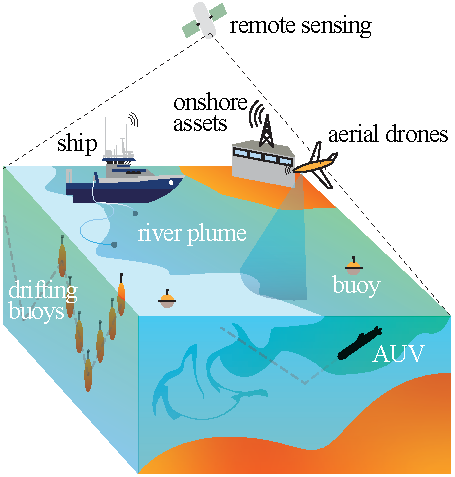
\includegraphics[width =
    0.48\textwidth]{Figures/envir.pdf}\label{fig:envir1}}
  \hfill
  \subfigure[Different coastal processes directly or indirectly
  associated with gradients and boundaries.]{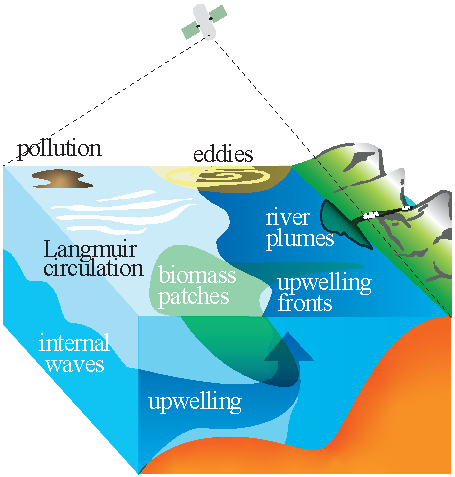
\includegraphics[width =
    0.48\textwidth]{Figures/envir_ocean.pdf}\label{fig:envir2}}
  \caption{Ocean observation is moving away from single-ship sampling
    towards more collaborative networked operations in order to resolve
    the numerous processes and their interaction.} \label{fig:envir}
\end{figure}

Our focus in this work is limited to spatial characterization of a river
plume system. Fig. \ref{fig:river_fronts} shows the survey area (the
outlet of the Nidelva river, Trondheim, Norway) taken as cold freshwater
enters from the river showing the separation of water masses and strong
gradients for both temperature and salinity. Because of the local
topography and the Coreolis force \citep{coriolis1835memoire} the cold
fresh water tends to stay near land to the east. Depending on the river
discharge, tidal effects, and temperature differences, this boundary in
water masses will get distorted. Prior knowledge about the location and
evolution of these features is therefore highly uncertain, making
deterministic planning sub-optimal.% , and one would rather demonstrate the
% ability of AUVs to map the plume area efficiently.

\begin{figure}[!h]
\centering
 % \subfigure[River front - Columbia River, Astoria, Oregon, US.]{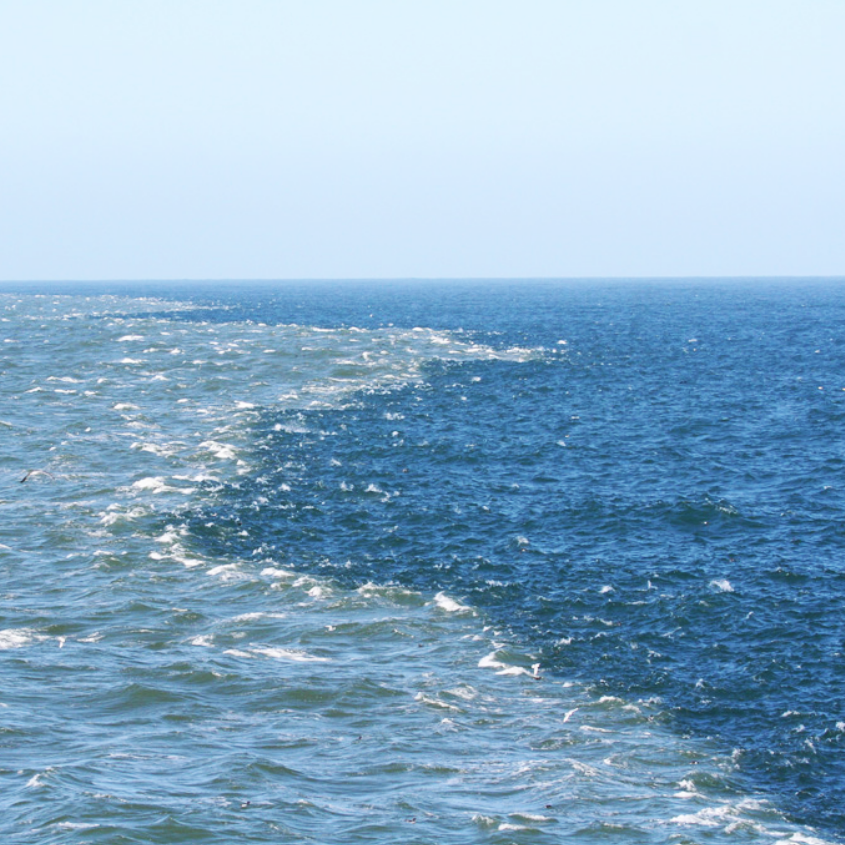
\includegraphics[width = 0.45\textwidth]{Figures/pictures/a.png}\label{fig:river1}}
 % \hfill
 \subfigure[Tidal front - Korsfjorden, Norway.]{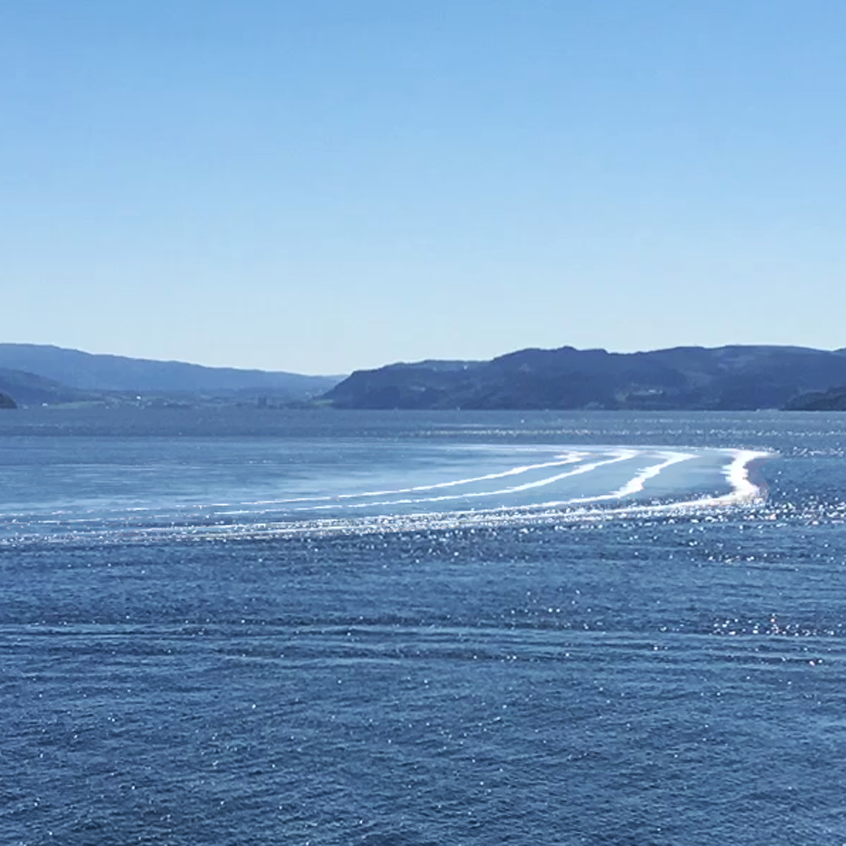
\includegraphics[width = 0.45\textwidth]{Figures/pictures/d.png}\label{fig:river2}}
 % \hfill
 % \subfigure[River plume - Rio de la Plata, Buenos Aires, Argentina.]{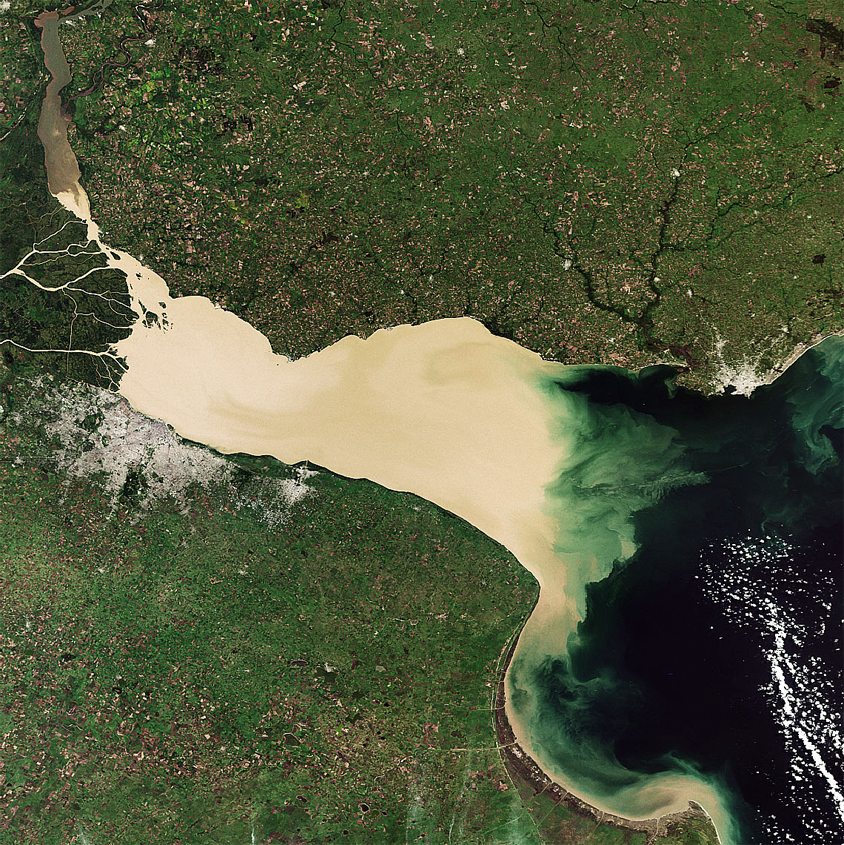
\includegraphics[width = 0.45\textwidth]{Figures/pictures/b.png}\label{fig:river3}}
 % \hfill
 \subfigure[Frontal patterns - Nidelva, Trondheim, Norway.]{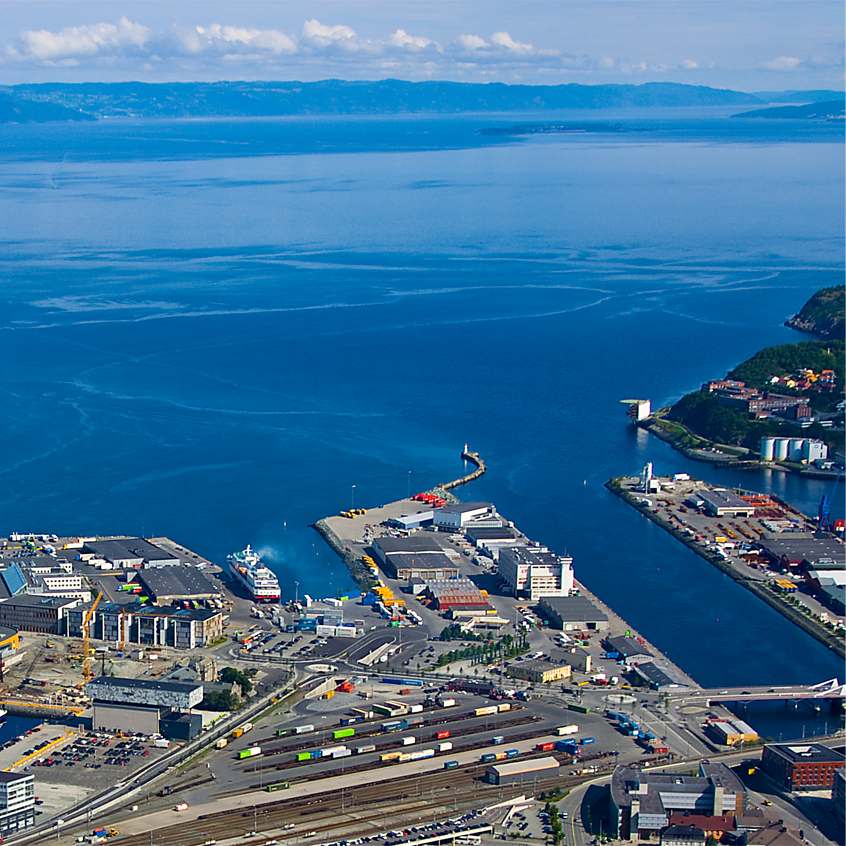
\includegraphics[width = 0.45\textwidth]{Figures/pictures/c.png}\label{fig:river4}}
 \caption{Two examples of frontal features associated with
   river-ocean interaction. % (\ref{fig:river1}) The river plume front of
   % the Columbia River meeting the Pacific Ocean.
   (\ref{fig:river2})  Superimposed images (over 10 minutes) of a surface tidal front in
   Korsfjorden, Norway. % (\ref{fig:river3}) The river plume of the Rio de
   % la Plata, taken by European Space Agency (ESA)'s Envisat platform and
   % MEdium Resolution Imaging Spectrometer (MERIS) sensor.
   (\ref{fig:river4}) Aerial image of the mouth of the Nidelva river in
   Trondheim, Norway where fresh water meets the salty fjord and creates
   frontal patterns.} % Image courtesy: (\ref{fig:river1})
   % \cite{zamon2014marine}, (\ref{fig:river3}) ESA, CC BY-SA 3.0 IGO.}
 \label{fig:river_fronts}
\end{figure}

%The use of \emph{robotic sampling} is motivated by the fundamental challenges of ocean observation, where a limited set of resources, a highly dynamic ocean, and the associated 

%This challenge can be addressed by employing more elaborate and adaptive sampling strategies that can capitalize on both prior and current observations in order to locate and map these areas.  

River plumes belong to a class of ocean processes that are local and
usually act on smaller \emph{sub-mesoscale}, from 10 m -- 5 km where
spatial lateral variability tends to dominate. Remote sensing and
synthetic ocean models find it challenging to provide detailed at this
scale \citep{Lermusiaux:2006} and the principal way to resolve for fine
resolution is by direct observation. At larger \emph{mesoscale} ($>50$
km), both three-dimensional space and time dynamics are important and
can shift substantially, while in the case of river plumes one can often
limit scope to cover only lateral spatial elements ([north, east]
domain). For this case, time-effects can be regarded as static when
acquiring AUV data over a short time window and limited region. However,
the methodological framework can be extended to three-dimensional
spatial variability and temporal elements in a similar manner.

\subsection{Autonomous Vehicles}

AUVs operate underwater used to gather spatio-temporal data from a
targeted domain, carrying a scientific payload to survey the water
column or the seafloor. They run at $\sim 1-3$ m/s, can reach depths
from 100--6000m. In water staying capacity depends on survey speed,
payload sensors and mission design. By deploying AUVs one can in
principle fill gaps and augment data obtained from either ocean models,
earth observing satellite data, or fixed-location sensors on buoys due
to their speed and mobility. Traditional operations and surveys with
AUVs are usually limited to planning samples along fixed transects or
survey lines set by human operators, programmed as a sequential plan
consisting of different waypoints and depths. But by using on-board
algorithms to continuously evaluate, update, and refine future sampling
locations, making information gathering adaptive \citep{das11b} is
feasible. For instance, an AUV could reconstruct or modify a survey line
based on what temperatures it is measuring by using embedded methods in
decision-theoretic planning \citep{ryan10}.

%To improve the state of sampling, modern tools and methods, including the use of autonomous platforms, oceanographic models and satellite remote sensing, needs to be combined with traditional data acquired by surface vessels or buoys (See Fig. \ref{fig:envir}). However, without adequate understanding of the theoretical underpinnings of how, when, and where to gather data, these tools and methods are insufficient in the vast and harsh oceans.

% retaining an advantageous strategy for information recovery, online during execution.
%The pressure on marine resources is growing and increased accuracy, resolution, and persistent monitoring of the oceans is crucial for long-term sustainable management. The impact of this research provides cost effective tools, techniques, and processes for doing ocean based measurements using robotic platforms. 
%adaptive design of experiments using robotic assets identifying and prioritizing relevant sampling locations on an information-theoretic basis. Spatial statistics naturally enters here through the ability to both model spatially correlated parameters and provide formal measures of uncertainty, on which this basis can be formed. 
%for oceanic sensing applications, where sensors are sparsely distributed and capitalizing on all available information is 

%This imperfect understanding of causality coupled with uncertainty implies that we need to obtain more measurements and use statistical models and methods to determine what and how phenomena form, to increase the quality of predictive statements. To improve the state of sampling, modern tools and methods, including the use of autonomous platforms, oceanographic models and satellite remote sensing, augment the more traditional data acquired by surface vessels or buoys (See Fig. \ref{fig:envir}). However, without adequate understanding of the theoretical underpinnings of how, when, and where to gather data, these tools and methods are insufficient in the vast and harsh oceans.

%There are several oceanographic data sources that can be used together with statistical tools to improve data collection in ocean science. In the following section we briefly discuss buoy data, satellite data, ocean models data, and AUV data.

%Buoy data provide very accurate information of oceanographic variables, but in most situations they are local, giving information only at one (north, east) coordinate, possibly with opportunities for conducting measurements at different depths. Gliders and other surface vessels are a kind of floating buoys that drift and can measure variables at many locations, but still with limited spatial coverage. 

%Satellite data are important for the mapping of oceanographic variables. They can also be indicative of variables such as temperature and salinity which we look at here, especially if the data are calibrated to for instance buoy data from the same spatial domain. However, the resolution of satellite data is relatively large, say $1 \times 1$ km $^2$ grid cells, and it only provides accurate information at the sea surface. Moreover, one cannot get useful satellite information on a cloudy day. 

%What is often done in practice is to run ocean models based on the complex differential equations governing oceanographic phenomena, where also satellite data can be assimilated and used as input, and possibly playing with different forcing mechanisms to capture some of the uncertainty of the models. Initial conditions, and can be used t the goal is to guide the sampling towards regions these regions, where we can reduce the uncertainty in the ES. These models provide insight that can be understood from practitioners, but they tend to be biased, and must also be calibrated to buoy data in one way or the other.

%to provide an effective specification of regions of phenomenological interest resolving the boundaries and the position of phenomena, on which evaluation of future sampling can be constructed.

%; some of these phenomena are illustrated in Fig. \ref{fig:envir2}. Figure \ref{fig:river_fronts} illustrates the %phenomena of interest in this paper, which is river plumes and their interaction with the ocean.

%Feature driven sampling
%processes acting across a wide range of spatio-temporal scales makes prioritizing sampling efforts necessary. %Autonomous robotic platforms, can address these issues by providing the ability to focus sampling efforts to %high-interest regions (``hotspots").


Determining paths for mobile robotic sensors in order to maximize the
information gained about an environment is formally known as informative
path planning. This, and related problems such as the orienteering
problem \citep{Golden87}, has been studied in the context of graphs,
where the potential measurement are assigned to nodes on which
evaluation of different routes can be conducted.
%In this context, a fundamental result from \cite{nemhauser1978analysis} proves that a simple greedy algorithm (iteratively selecting the location which most increases the utility) can achieve a near-optimal solution if the problem can be shown to be \emph{submodular}\footnote{an intuitive diminishing returns property, where the informative value of adding sensors decrease with the number of sensors added.}. Building on this result, \cite{chekuri2005recursive} explored this in the setting of a graph using a recursive greedy algorithm, providing near-optimal solutions depending on the planning horizon and graph resolution. 
Adaptive sampling of an evolving frontal feature has been explored in \cite{Zhang2012} and \cite{Pinto2018} using state-based autonomous agents. Both approaches use a reactive-adaptive scheme, meaning that the selection does not use a statistical model of the environment in its strategic sampling effort, but rather adapts based on detection and state switching.
Myopic sampling, i.e. step-wise selection of the path (on the graph) which reduces the information criterion the most, has been used for adaptive surveying \citep{singh2009efficient,Binney2013}. These exploration strategies focus largely on reducing predictive variance or mutual information (entropy). Because the variance and entropy reduction are independent of the actual data realizations under the assumption of GP models, the use of data-driven (adaptive) criteria was introduced to include more targeted sampling of interesting regions (hotspot sampling) by \cite{Low2009} and \cite{fossuminformation}. 


%\begin{figure}[h]
%\centering
%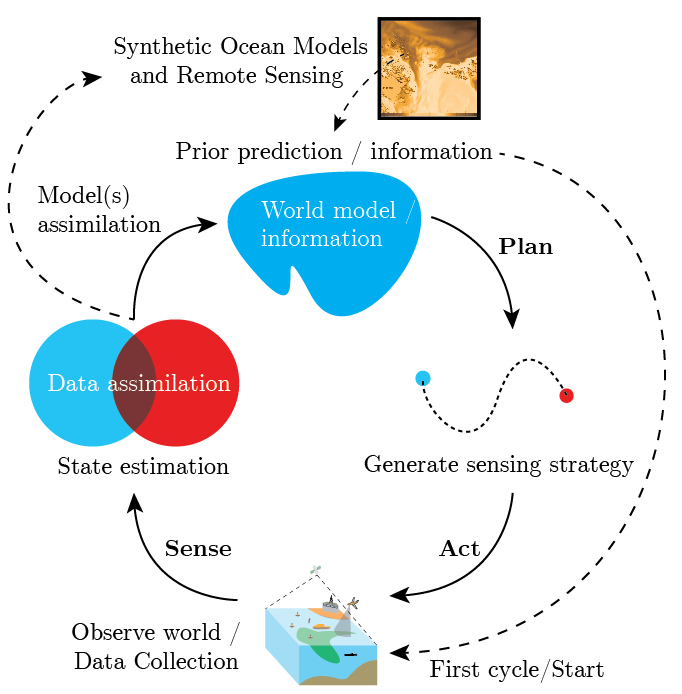
\includegraphics[width=0.4\textwidth]{Data-driven.png}
%\label{fig:auv_alone}
%\caption{The concept of data-driven sampling.}
%\end{figure}

%The goal is effectively map the extension of the river plume given this


%, we can formulate this question as follows: the ocean region  defined by the boundary between water bodies, separated by a characteristic temperature gradient that is smaller than $T=5$\textdegree C and a salinity concentration lower than $S=30$ [g/kg]. A goal is then to improve our predictive capabilities to answer this question better.
%For example,  (examples are shown in Fig. \ref{fig:river_fronts}). However, 

% In doing so, the aim is to increase the knowledge about the uncertain ocean environment through adaptive sampling


\subsection{Notation and excursion sets}

In our setting we study two variables; temperature and salinity, which together characterize the phenomenon taking place in the river plume. At location $\bx \in \mathcal{M} \subset \mathbf{R^2}$, we define the two process variables by $\bxi(\bx)=(\xi_a(\bx),\xi_b(\bx))$. %In practice there is of course time variability, but we assume this to be negligible during the AUV operation. Depth variability could also be important in some cases, but in the current application the with depths only a few meters this is considered irrelevant for mapping the phenomenon. 

In the context illustrated by Figure \ref{fig:river4}, interest is on spatial separation of cold freshwater. 
Because a main goal is classifying the water masses, ES variability is a useful sampling criterion for guiding the observation effort of the AUV. 
A bivariate ES is here defined via joint variables being below thresholds, at individual locations, for the process over the spatial domain $\mathcal{M}$.
Denoting the threshold for temperature by $T_a$ and the threshold for salinity by $T_b$,
we use the following definition;
 \begin{equation}\label{ES}
     \mbox{ES} = \{\bx \in \mathcal{M} | \xi_a(\bx) < T_a,\xi_b(\bx) < T_b\}.
 \end{equation}
The excursions could also be defined as larger than threshold, or within a boundary of limits for the two variables. Calculations and interpretations will be similar in these different cases. 

The ES is defined by random indicator variables, and the associated EPs become 
\begin{equation}\label{eq:prob}
 p(\bx) = P(\xi_a(\bx) < T_a, \xi_b(\bx) < T_b), \hspace{3mm} \bx \in \mathcal{M}.
\end{equation}
The actual calculation of the EP would require a model specification. As we demonstrate below, Gaussian modeling assumptions facilitate the computation. 
If the EPs in Eq. (\ref{eq:prob}) are close to $1$ or $0$, it is easy to classify water masses. It is more difficult if the probabilities are close to $0.5$. In this case it will likely be worthwhile gathering data to improve the classification skill. 

There has lately been much statistical literature on ESs and EPs connected to spatial statistics \citep{french2013spatio,bolin2015excursion,french2016credible}. 
Most of the work done is based on GPs for the spatial phenomenon, as we use here.
Our focus in the current paper is on ES as defined in Eq. (\ref{ES}) and location-wise EPs and the uncertainty reduction that can be achieved by informative sampling. 
In this sense our work is similar to \cite{chevalier2014fast} and \cite{azzimonti2016quantifying} who described analytical results for uncertainty reduction in ESs for univariate processes.
One contribution of the current paper is to derive closed-form results for expectations of ESs in the situation with multivariate processes.

\section{Gaussian processes and excursion probabilities}\label{sec:GP_EP}


\subsection{Bivariate Gaussian processes}

We represent the bivariate random field of ocean temperature and salinity by a Gaussian model.
At location $\bx \in \mathcal{M}$, the bivariate distribution is 
\begin{equation}\label{gp_bar}
\begin{bmatrix}\xi_a(\bx) \\
\xi_b(\bx) 
\end{bmatrix}
 \sim N \left( 
\begin{bmatrix} \mu_{a}(\bx)\\
\mu_{b}(\bx)
\end{bmatrix},\begin{bmatrix}
\sigma_{a}^2(\bx) & \sigma_{a}(\bx) \sigma_b(\bx) \gamma  \\
\sigma_{a}(\bx) \sigma_b(\bx) \gamma  & \sigma_{b}^2(\bx) 
\end{bmatrix}
\right).
\end{equation}
Here, the means and standard deviations are allowed to vary with location, which can be important for capturing the trends and variabilities near a river mouth. The correlation in salinity and temperature is assumed to be the same for all locations.

There exist several multivariate spatial covariance functions \citep{gneiting2010matern,genton2015cross}. But in practice it has shown difficult to estimate all parameters from data. Like is often done, we assume the same correlation decay for salinity and temperature, which is not unrealistic for a river plume. We use a separable covariance function such that
\begin{eqnarray}\label{gp_corr}
\mbox{Cov}(\xi_a(\bx),\xi_b(\bx')) &=& \rho(\bx,\bx') \gamma \sigma_a(\bx) \sigma_b(\bx'), \\
\mbox{Cov}(\xi_a(\bx),\xi_a(\bx')) &=& \rho(\bx,\bx') \sigma_a(\bx) \sigma_a(\bx'), \nonumber \\
\mbox{Cov}(\xi_b(\bx),\xi_b(\bx')) &=& \rho(\bx,\bx') \sigma_b(\bx) \sigma_b(\bx'). \nonumber
\end{eqnarray}
Moreover, we assume a stationary isotropic correlation function $\rho(\bx,\bx')=\rho(h)$, for distance $h=\sqrt{(\bx-\bx')^t (\bx-\bx')}$.

For implementation on the computer, we discretize the spatial domain $\mathcal{M}$ on a set of $n$ grid locations; $\mathcal{M}_g = \{\bx_i, i=1,\ldots,n \}$.
We let $\Delta$ be the area of each cell in the regular grid.
Using vector notation, we collect the temperature and salinity variables on the grid as
\begin{equation}
    \bxi=(\xi_a(\bx_1),\xi_b(\bx_1),\ldots,\xi_a(\bx_n),\xi_b(\bx_n))^t \sim \mbox{GP} (\bmu,\bSigma), \nonumber
\end{equation}
where the entries in length $2 n$ vector $\bmu$ hold the expected values of temperature and salinity at the grid locations, and the $2n \times 2n$ matrix $\bSigma$ holds all the covariances between temperature and salinity variables at all grid locations. 
 The joint probability density function is then
\begin{equation}\label{prior}
\pi(\bxi) = N(\bxi;\bmu,\bSigma) = \frac{1}{(2\pi)^{\frac{n}{2}}|\bSigma|^{\frac{1}{2}}}e^{-\frac{1}{2}(\bxi -\bmu)^T\bSigma^{-1}(\bxi - \bmu)}.
\end{equation}


\subsection{Updating Gaussian processes}

The GP mean and covariance in Eq. (\ref{prior}) are updated when more information gets available. 
In our setting, the autonomous vehicle will collect a batch of temperature and salinity measurements along a survey path. After each batch, the data are assimilated to get an updated model.
We here describe one round of updating. In Section \ref{sec:heuristics} we discuss sequential data gathering and model updating.

Denote the AUV data at $m$ locations by $\by=(y_{a,1},y_{b,1},\ldots,y_{a,m},y_{b,m})^t$, representing the temperature and salinity measurements gathered along a survey line.
Restricting attention to the grid representation, the likelihood model is described by 
\begin{equation}\label{likelihood}
\by | \bxi \sim GP(\by; \bA \bxi,\bR),
\end{equation}
where $\bA$ is an $2m \times 2n$ matrix holding $1$ entries at the measurement indexes on the grid, and otherwise $0$ entries. The size $2m \times 2m$ covariance matrix $\bR$ is diagonal with entries $r_a$ and $r_b$ which are the measurement error variances of temperature and salinity observations. 

The updated distribution for temperature and salinity variables on the spatial grid, given survey data $\by$, is Gaussian with mean and covariance
\begin{eqnarray}\label{gp_upd}
\bm &=& \bmu+\bSigma \bA^t (\bA \Sigma \bA^t+\bR)^{-1}(\by-\bA \bmu),  \\
\bS &=& \bSigma - \bSigma \bA^t (\bA \bSigma \bA^t+\bR)^{-1} \bA \bSigma.\nonumber
\end{eqnarray}
The updated bivariate distribution at a grid location $\bx$ is then 
\begin{equation}\label{gp_hat}
\begin{bmatrix}
\xi_a(\bx) \\
\xi_b(\bx)
\end{bmatrix}
 |\by
 \sim N \left( 
\begin{bmatrix} m_{a}(\bx)\\
m_{b}(\bx)
\end{bmatrix},\begin{bmatrix}
s_{a}^2(\bx) & s_{a,b}(\bx)  \\
s_{a,b}(\bx)  & s_{b}^2(\bx)  
\end{bmatrix}
\right),
\end{equation}
with entries extracted from the conditional mean and covariance expressions in Eq. (\ref{gp_upd}).

The conditional mean $\bm$ will be important in the following derivation in Section \ref{sec:sur}. This mean is a linear function of the data $\by$, and since the marginal distribution of the data is $\by \sim N( \bA \bmu,\bA \bSigma \bA^t+\bR)$, we get
\begin{equation}\label{distxi}
\bm \sim N(\bmu , \bPsi), \hspace{3mm} \bPsi=\bSigma \bA^t (\bA \bSigma \bA^t+\bR)^{-1} \bA \bSigma.  
\end{equation}
When considering only grid location $\bx$, we can extract elements from the mean vector and covariance matrix to get the bivariate distribution as follows 
\begin{equation}\label{dist_mxi}
\bm(\bx) \sim N 
\left( 
\begin{bmatrix}
\mu_{a}(\bx) \\
\mu_{b}(\bx)
\end{bmatrix},
\begin{bmatrix}
\psi^2_{a}(\bx) & \psi_{a,b}(\bx)\\
\psi_{a,b}(\bx) & \psi^2_{b}(\bx)
\end{bmatrix}
\right).
\end{equation}


\subsection{Excursion probabilities for Gaussian processes}

Based on the Gaussian modeling assumptions, the EPs in Eq. (\ref{eq:prob}) can be computed at any location $\bx$. Without additional data, we have
\begin{eqnarray}\label{eq:prob_mv0}
 p(\bx) &=& P(\xi_a(\bx) < T_a, \xi_b(\bx) < T_b) \nonumber \\
 &=& \Phi_2 \begin{pmatrix} 
\begin{bmatrix} T_a\\
T_b
\end{bmatrix};
\begin{bmatrix} \mu_{a}(\bx)\\
\mu_{b}(\bx)
\end{bmatrix},\begin{bmatrix}
\sigma_{a}^2(\bx) & \sigma_{a}(\bx)\sigma_{b}(\bx) \gamma  \\
\sigma_{a}(\bx)\sigma_{b}(\bx) \gamma  & \sigma_{b}^2(\bx)  
\end{bmatrix}\end{pmatrix},
\end{eqnarray}
where $\Phi_2$ is the bivariate Gaussian cumulative distribution function, and the mean and covariance entries are defined in Eq. (\ref{gp_bar}). 

When data $\by$ is available, we similarly get
\begin{eqnarray}\label{eq:prob_mv}
 p(\bx;\by) &=& P(\xi_a(\bx) < T_a, \xi_b(\bx) < T_b |\by) 
 \nonumber \\
 &=& \Phi_2 \begin{pmatrix} 
\begin{bmatrix} T_a\\
T_b
\end{bmatrix};
\begin{bmatrix} m_{a}(\bx)\\
m_{b}(\bx)
\end{bmatrix},\begin{bmatrix}
s_{a}^2(\bx) & s_{a,b}(\bx)  \\
s_{a,b}(\bx)  & s_{b}^2(\bx)  
\end{bmatrix}\end{pmatrix},
\end{eqnarray}
with parameters defined in Eq. (\ref{gp_upd}) and (\ref{gp_hat}). 

For one particular dataset, the probability $p(\bx;\by)$ can be closer to $0.5$ than the initial probability $p(\bx)$. This means that the variance in the ES is increased. On average, taking expectations over the data $\by$, the ES variance will be reduced by gathering data. We next explain how AUVs can be used to efficiently gather data and reduce the overall marginal spatial uncertainties in the ES. 

\section{Uncertainty reduction on excursion sets}\label{sec:sur}

\subsection{Variance in excursion set}

Regions with temperatures or salinity that surpasses the thresholds with a large margin (e.g. very high/low temperatures) are not interesting, unless the uncertainty at these locations is very large. The objective will therefore be to explore regions where the process variables are close to the thresholds. With this mind, it is valuable to explore locations $\bx$ where $p(\bx) \approx 0.5$. This is what gives the maximum variance $p(\bx) (1-p(\bx))$ in the indicator for the ES. 

Consider then a measure as follows:
\begin{equation}\label{measVAR}
    V = \int_{\bx \in \mathcal{M}} p(\bx) \left(1-p(\bx)\right) d\bx \approx \sum_{x \in \mathcal{M}_g} p(\bx) \left(1-p(\bx)\right) \Delta.
\end{equation}
The measure is dominated by location having probabilities close to $0.5$. 

Considering one location only, we study the effect of different correlation $\gamma$ and prior variance. 
Figure \ref{illus_bivarDens} shows contour plots of three different densities. Here, the temperature mean is $T_a=5^o$ and salinity mean is $T_b=30$ mg/l. The thresholds are identical to these means. The variables have unit variance and different correlation (low, medium and high).
\begin{figure}[h!]
\centering
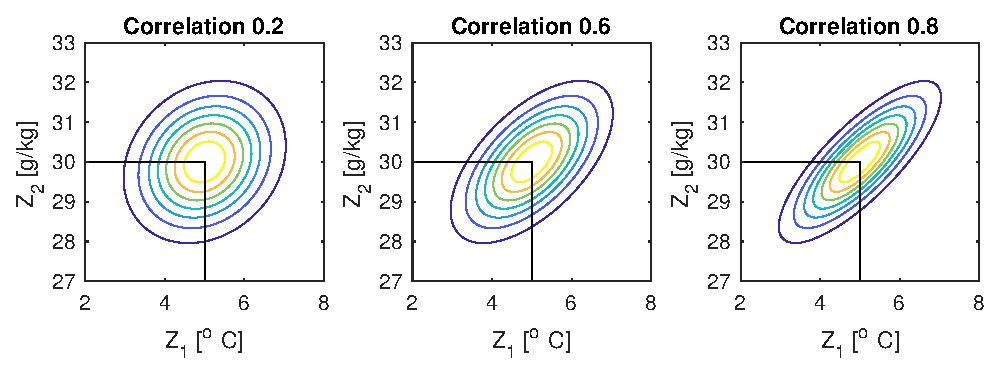
\includegraphics[width=0.99\textwidth]{Figures/illus_bivar.eps}
\caption{Density contour plots having different correlations for temperature and salinity.}\label{illus_bivarDens}
\end{figure}
Table \ref{tab:sim_rhoab} shows the EPs and the associated variances in the ES (top rows). The results are computed for different correlations $\gamma$ indicated in Figure \ref{illus_bivarDens}, and for standard deviations $1$ (left) and $2$ (right). The variance in the ES is largest for high correlation, as there is more tendency of joint small or high occurrences for temperature and salinity in this case. EPs are the same for standard deviation $1$ or $2$. 
\begin{table}[!h]
\centering
\caption{EP and variance of ES for different correlations (top rows), and for data of both variables and only for temperature (bottom rows).}
\begin{tabular}{c|ccc|ccc}
 &\multicolumn{3}{c}{$\sigma_b=\sigma_a=1$} & \multicolumn{3}{c}{$\sigma_b=\sigma_a=2$} \\
\hline
Correlation $\gamma$ & 0.2 & 0.6 & 0.8 & 0.2 & 0.6 & 0.8 \\
\hline
$p$ & 0.28 & 0.35 & 0.40 & 0.28 & 0.35 & 0.40 \\ 
$p(1-p)$ & 0.20 & 0.23 & 0.24 & 0.20 & 0.23 & 0.24 \\ 
$E_{(y_a,y_b)}(p (1-p))$ & 0.092 & 0.089 & 0.085 & 0.052 & 0.051 & 0.049 \\ 
$E_{y_a}(p (1-p))$ & 0.151 & 0.138 & 0.123 & 0.137 & 0.114 & 0.093 \\ 
\hline
\end{tabular}
\label{tab:sim_rhoab}
\end{table}

\subsection{Expected variance criteria}

When designing AUV sampling paths, we aim to reduce the variances in the ES and in this way efficiently characterize the ES throughout the spatial domain. We saw that the measure defined by Eq. (\ref{measVAR}) does not discriminate between high or low variability in the temperature and salinity (two top rows of Table \ref{tab:sim_rhoab}).
Also, focusing only on locations with EPs near $0.5$ would not account for the spatial correlation in the model.  
The same has been seen for related measures learning graphical models \citep{lilleborge2016information}.

To evaluate AUV data sampling paths, it is hence natural to evaluate the expected variance reduction in the ES  \citep{chevalier2014fast}, as provided by the survey data. In this way, we take the expectation with respect to the planned measurements $\by$:
\begin{eqnarray}\label{sur}
    V_{\mbox{upd}} &=& \int_{\bx \in \mathcal{M}} E_{\by} \left\{ p(\bx;\by)\left( 1-p(\bx;\by)\right) \right\} d\bx \\
    & \approx & \sum_{\bx \in \mathcal{M}_g} E_{\by} \left\{ p(\bx;\by)\left( 1-p(\bx;\by)\right) \right\} \Delta, \nonumber \\
    p(\bx;\by) &=& P(\xi_a(\bx) < T_a, \xi_b(\bx) < T_b |\by), \nonumber
\end{eqnarray}
where the conditional probability is defined in Eq. (\ref{eq:prob_mv}).

We will next derive closed form solutions to the expectation in (\ref{sur}). A critical
element in the derivation is the GP model, and the linear dependence on data $\by$, which means that we have a closed form Gaussian distribution for the conditional mean in Eq. (\ref{dist_mxi}). This means that the high-dimensional inner integral in Eq. (\ref{sur}) reduces to a univariate integral \citep{bhattacharjya2013value, chevalier2014fast}. 

Table \ref{tab:sim_rhoab} (bottom two rows) shows results of doing such calculations, for different correlation $\gamma$ and standard deviations (left and right). Here, the expected variances are computed for both data types $(y_a,y_b)$, and for temperature measurements $y_a$ alone. With both data; $(y_a,y_b)^t=(\xi_a,\xi_b)^t+N(0,0.5^2\bI)$, while $y_a=\xi_a+N(0,0.5^2)$ when only temperature is measured.
The results in Table \ref{tab:sim_rhoab} shows that 
the expected variance depends on the (prior) uncertainty in temperature and salinity. The expected variance in the ES is lower with larger standard deviations $\sigma_a$ and $\sigma_b$ (right columns). Moreover, the relative reduction is largest for the case with high correlation $\gamma$. There is also large uncertainty reduction when only temperature is measured (bottom row), especially when the temperature and salinity are very dependent. When correlation is low ($\gamma=0.2$) there is hardly any information about salinity in the temperature data. In the application with fresh cold water from the river, the temperature and salinity variables will not only be interdependent, but they will be dependent in the spatial dimension, so this kind of location-wise dependence will also impact design criteria when we evaluate the information measure by integrating over several locations $\bx$. 

\subsection{Analytical results for bivariate ES}

In the rest of this section, the location index $\bx$ is suppressed to avoid overly complex notation. We present new results for computing the expectation $E_{\by}\left\{ \cdot \right\}$ which is the integrand of Eq. (\ref{sur}).

The first key result is that the expectation only depends on the data through the linear combination $\bm=(m_{a},m_{b})^t$. 
To see this we standardize the two variables i.e.
$Z_a=\frac{\xi_a-m_{a}}{s_{a}}$,
$Z_b=\frac{\xi_b-m_{b}}{s_{b}}$; 
then
\begin{eqnarray}
   P(\xi_a < T_a, \xi_b < T_b|\by) &=& P \left( Z_a <\frac{T_a-m_{a}}{s_{a}}, Z_b <\frac{T_b-m_{b}}{s_{b}}|\by \right) \nonumber \\
   &=& \Phi_2 \begin{pmatrix} 
\begin{bmatrix} \frac{T_a-m_{a}}{s_{a}}\\
\frac{T_b-m_{b}}{s_{b}}
\end{bmatrix};
 \begin{bmatrix} 0\\
0
\end{bmatrix},\begin{bmatrix}
1 & \eta_{s,t}  \\
\eta_{s,t}   & 1  
\end{bmatrix}\end{pmatrix} \nonumber \\
&=& P(\xi_a < T_a, \xi_b < T_b|\bm),
\end{eqnarray}
where $\eta_{a,b} =s_{a,b}/(s_{a} s_{b})$ is defined in Eq. (\ref{eq:prob_mv}).
Since the expression only depends on $\by$ via $\bm$, the expectation in Eq. (\ref{sur}) is reduced to a bivariate integral over $\bm$ (which will vary for each integrand term, because the locations differ). 

The expected variance can now be written as
\begin{eqnarray}\label{eq:var2}
E_{\by}(p[1-p]) &=& E_{\bm}(p[1-p]), \hspace{3mm} p=P(\xi_a < T_a, \xi_b < T_b|\bm) \nonumber \\
E_{\bm}(p[1-p]) & = & \int p[1-p] p(\bm) d\bm, \nonumber \\
 &=& \int P(\xi_a < T_a, \xi_b < T_b|\bm)  p(\bm) d\bm \nonumber  \\
&-& \int P(\xi_a < T_a, \xi_b < T_b|\bm) P(\xi_a < T_a, \xi_b < T_b|\bm) p(\bm) d\bm, 
\end{eqnarray}
where the integral is split in two components.
We will next extend results of \cite{chevalier2014fast} to solve for these two parts.

Considering part I of expression (\ref{eq:var2}), we have
\begin{equation}\label{part1:phi2}
 \int P(\xi_a < T_a, \xi_b < T_b|\bm) p(\bm) d\bm= 
P \left( Z_{a} < \frac{T_a-m_{a}}{s_{a}}, 
Z_{b} < \frac{T_b-m_{b}}{s_{b}} \right), \nonumber
\end{equation}
where $\bZ=(Z_{a},Z_{b})$ is a bivariate zero-mean and unit-variance Gaussian vector, with $\mbox{Corr}(Z_{a},Z_{b})=\eta_{a,b}$. Moreover, $\bZ$ is chosen to be independent of $\bm$. Using Eq. (\ref{dist_mxi}) we have
\begin{equation}
    E(s_{a} Z_{a}+m_{a}-T_a) = \mu_{a}-T_a, \hspace{3mm}
    \mbox{Var}(s_{a} Z_{a}+m_{a}-T_a) = s^2_a+ \psi^2_{a}, 
\end{equation}
and the same holds for the salinity part with subscript $b$. From this calculation, we get
\begin{eqnarray}\label{two_parts0}
& P & \left( Z_{a} < \frac{T_a-m_{a}}{s_{a}}, 
Z_{b} < \frac{T_b-m_{b}}{s_{b}} \right) \\
&=& \Phi_2 \begin{pmatrix} 
\begin{bmatrix} 0\\
0
\end{bmatrix};
\begin{bmatrix} \mu_{a}-T_a\\
\mu_{b}-T_b
\end{bmatrix},\begin{bmatrix}
s^2_a+ \psi^2_{a} & s_{a,b}+\psi_{a,b}  \\
s_{a,b}+\psi_{a,b}   & s^2_a+ \psi^2_{a} 
\end{bmatrix}\end{pmatrix} \nonumber.
\end{eqnarray}

For part II of expression (\ref{eq:var2}), standardization means that
\begin{eqnarray}\label{part1:phi4}
&& \int P(\xi_a < T_a, \xi_b < T_b|\bm) P(\xi_a < T_a, \xi_b < T_b|\bm) p(\bm) d\bm_{\xi}= \nonumber \\
&& P\left( Z_{1,a} < \frac{T_a-m_{a}}{s_{a}}, 
Z_{1,b} < \frac{T_b-m_{b}}{s_{b}},Z_{2,b} < \frac{T_a-m_{a}}{s_{a}}, 
Z_{2,b} < \frac{T_b-m_{b}}{s_{b}} \right). \nonumber
\end{eqnarray}
Here,
$\bZ_1=(Z_{1,a},Z_{1,b})$, $\bZ_2=(Z_{2,a},Z_{2,b})$ are independent bivariate zero-mean and unit-variance Gaussian vectors, both with element-wise correlation
$\eta_{a,b}$. Moreover, $\bZ_1$ and $\bZ_2$ are chosen to be independent of $\bm$. Hence,
\begin{equation}
    \left(
    \begin{array}{cccccc}
         Z_{1,a} \\
         Z_{1,b} \\
         Z_{2,a} \\
         Z_{2,b} \\
         m_{a} \\
         m_{b}
    \end{array}
    \right)
\sim N \left(
\left(
    \begin{array}{cccccc}
    0 \\
    0 \\
    0 \\
    0 \\
          \mu_{a} \\
         \mu_{b} 
    \end{array}
    \right),
   \left[ 
      \begin{array}{cccccc}
        1 & \eta_{a,b} & 0 & 0 & 0 & 0  \\
        \eta_{a,b} & 1 & 0 & 0 & 0 & 0 \\
        0 & 0 & 1 & \eta_{a,b} & 0 & 0 \\
        0 & 0 & \eta_{a,b} & 1 & 0 & 0 \\
        0 & 0 & 0 & 0 & \psi^2_{a} & \psi_{a,b} \\
        0 & 0 & 0 & 0 & \psi_{a,b} & \psi^2_{b} 
    \end{array}
\right]
\right).
\vspace{0.2cm}
\end{equation}

The solution to part II is then to evaluate a four-variable cumulative distribution function, accounting for the mean, variance and covariances of $\bZ_1$, $\bZ_2$ and $\bm$ in the appropriate linear combinations. Using vector-matrix formulations, we define linear combinations
\begin{equation}\label{Vcomb}
    \bV=\left[
    \begin{array}{cccccc}
        s_a & 0 & 0 & 0 & 1 & 0 \\
         0 & s_b & 0 & 0 & 0 & 1 \\
         0 & 0 & s_a & 0 & 1 & 0\\
         0 & 0 & 0 & s_b & 0 & 1\\
    \end{array}
    \right] 
    \left(
    \begin{array}{cccccc}
         Z_{1,a} \\
         Z_{1,b} \\
         Z_{2,a} \\
         Z_{2,b} \\
         m_{a} \\
         m_{b}
    \end{array}
    \right),
\end{equation}
and the part II calculation becomes
\begin{eqnarray}\label{part1:phi4}
&& P \left( Z_{1,a} < \frac{T_a-m_{a}}{s_{a}}, 
Z_{1,b} < \frac{T_b-m_{b}}{s_{b}},Z_{2,b} < \frac{T_a-m_{a}}{s_{a}}, 
Z_{2,b} < \frac{T_b-m_{b}}{s_{b}} \right)  \\
&=&  \Phi_4 
\begin{pmatrix} 
\begin{bmatrix} T_a\\
T_b \\
T_a \\
T_b
\end{bmatrix};
E( \bV),Var(\bV)
\end{pmatrix} \nonumber.
\end{eqnarray}

The multivariate cumulative probabilities in two and four dimensions are fast to compute using methods of \cite{genz2009computation}.
In the end, the part I solution in Eq. (\ref{two_parts0}) and part II solution in Eq. (\ref{part1:phi4}) are computed for each location on the grid, and summing over the spatial domain $x \in \mathcal{M}_g$, gives the design evaluation criterion in Eq. (\ref{sur}).


\subsection{Generalization to the multivariate case}

In our application with temperature and salinity, the solutions to the complex integral equations for the expected variance are reduced to calculating bi-variate and four-variate cumulative distribution functions for Gaussian vectors. For the more general situation one would be interested in $K$ random fields. Say, in the ocean sciences the variables could include chlorophyll or plankton variables, in addition to temperature and salinity. 

The equations derived in the previous section can be generalized to such $K$-variable cases. We then define $\bxi(\bx)=(\xi_1(\bx),\ldots,\xi_K(\bx))$, and the expected variance in the ES is
\begin{equation}\label{two_partsK}
E_y(p[1-p]) = \int p[1-p] p(\by) d\by, \hspace{3mm} P(\xi_k < T_k ; k=1,\ldots,K|\by). 
\end{equation}
By the first key result of linear combination of Gaussian variables, we reduce the integral to a $K$ dimensional integral of the relevant $\bm=E(\bxi(\bx)|\by)$. Next, reducing the integral to two parts, we standard the variables in each and compute cumulative distributions. 
In summary, we get 
\begin{equation}\label{two_parts}
E_y(p[1-p]) =  \Phi_K 
\begin{pmatrix}
\begin{bmatrix} T_1\\
\vdots \\
T_K 
\end{bmatrix};
\bmu,\bS+\bPsi 
\end{pmatrix}
- \Phi_{2K} 
\begin{pmatrix}
\begin{bmatrix} T_1\\
\vdots \\
T_K \\
T_1\\
\vdots \\
T_K 
\end{bmatrix};
E(\bV),Var(\bV) 
\end{pmatrix},\nonumber
\end{equation}
where $\bS$ and $\bPsi$ are direct $K$-variate extensions of the matrices entries in Eq. (\ref{two_parts0}), and the matrix $\bV$ finds the relevant linear combination of two independent vectors $\bZ_l=(Z_{l,1},\ldots,Z_{l,K})$, $l=1,2$ and $\bm$, as an extension of Eq. (\ref{Vcomb}).

%\subsection{Expected classification criteria}

%{\bf{I have not done anything here - skip this, I think}}.

%Rather than minimizing expected variance one can aim at minimizing the classification probability of the excursion set: 
%$\min [p,(1-p) ]$, see e.g. \cite{lilleborge2016information}. 

%Again, since the conditional mean is a linear in the data, we only have to look at the %relevant linear combination via $\bm_{\xi}=E(\bxi)$.
%See also \cite{bhattacharjya2013value}.

%\begin{equation}
%E(\min \{ p,(1-p)\})=\int \min P(\xi_a < t, \xi_b < s),[1-P(\xi_a < t, \xi_b < s)] p(E(\bxi)=) dE(\bxi)=,
%\end{equation}
%for the complementary probabilities, this is again evaluated by the corner regions for the block, and $\Phi_4()$ evaluations are required.

%In the end, this result is integrated over the spatial domain $x \in X$.

\section{Sequential updating and heuristic path planning}\label{sec:heuristics}

\subsection{Optimal sequential design}
\label{myopic}

The derived closed form solutions for the expected variance (in the multivariate ES) can now be used to evaluate and select among different survey designs for sampling applications with robotic platforms. 
Considering a set $\mathcal{J}$ of possible designs for a survey. A criterion for the AUV path selection is
\begin{equation}\label{crit}
    j^* = \mbox{argmin}_{j \in \mathcal{J}} V_{\mbox{upd}}(j),
\end{equation}
where the criterion $V_{\mbox{upd}}(j)$ in Eq. (\ref{sur}) is computed for each of the possible designs.
In practice, a survey is split in many stages, giving opportunities for sequential adaption of the AUV path. This means that the optimal survey design is found by considering not only the best current AUV line, but also what data gathered along this line would lead to for future sampling at the next stages. 

Let $d^{j,n}$ denote design number $j$ at stage $s$ of sequential surveying. If this design is selected, data $\by^{j,s}$ will be gathered. The optimal path selection situation is then depicted in Figure \ref{fig:PathSelOpt}, 
\begin{figure}[h!]
\centering
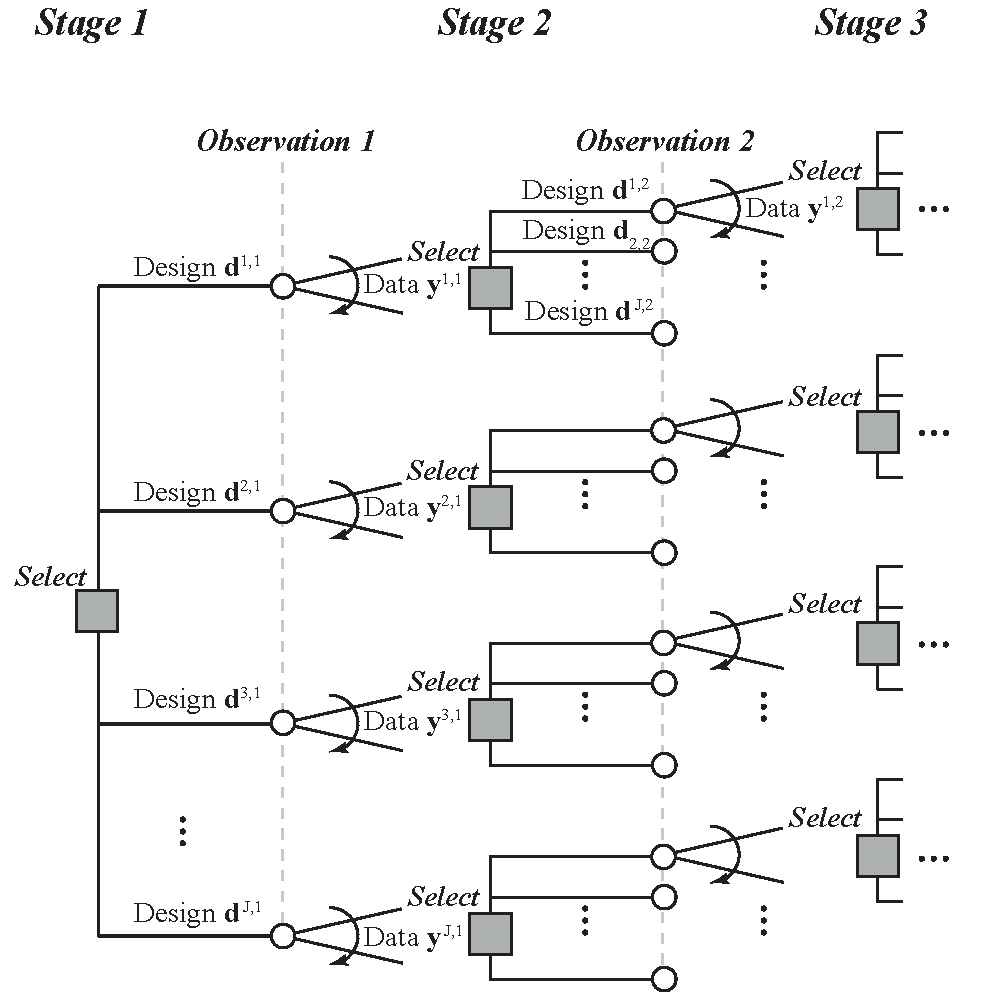
\includegraphics[width=0.85\textwidth]{Figures/sequent_select.pdf}
\caption{Optimal sequential path selection.}\label{fig:PathSelOpt}
\end{figure}
where design choices are indicated by squares while data realizations are indicated by circles. 
In mathematical terms this optimal design is defined as
\begin{equation}\label{opt_crit}
    \bd^* = \mbox{argmin}_{d^{j,1}} \left\{ \int_{\by^{j,1}} \mbox{argmin}_{d^{j,2}} \left\{ \int_{\by^{j,2}} \ldots p(\by^{j,2}|\by^{j,1}) d\by^{j,2} \right\} p(\by^{j,1}) d \by^{j,1} \right\},
\end{equation}
where $\ldots$ represents the expected variance reduction in the ES under the continued optimal design, which will depend on the data at earlier stages. 

In practice the optimal solution is not tractable because of the enormous growth in maximization and integral terms over stages, see e.g. \cite{sucar2015probabilistic} and \cite{powell2016perspectives}. Instead, we next outline two heuristic strategies. In terms of notation, let $\mathcal{Y}^{s-1} =\{d^{j,r}, \by^{j,r} ; r=1,\ldots,s-1 \}$ denote the data gathered until stage $s-1$, using a design indexed $j$ (which is suppressed in the data set $\mathcal{Y}^{s-1}$.

\subsection{Naive path planning}
\label{naive}

The simplest heuristic for adaptive sampling is to choose the next sampling location based on current EPs. The variance is largest for EP equal to $0.5$, so one selects the graph location where $\bx$ with average probabilities $p(\bx)$ closest to $0.5$. 

At stage $s$, based on the currently available data $\mathcal{Y}^{s-1}$, we fit an updated Gaussian model from Eq. (\ref{gp_upd}), with mean $\bm_{s-1}$ and covariance matrix $\bS_{s-1}$, represented on the grid locations covering the spatial domain. 
The next batch of measurements $\by^{j,s}$, can be  gathered with design $j=1,\ldots,J$, indicating all possible AUV lines at the current stage. The selected design is then
\begin{equation}\label{critNaive}
    d^{*,n} = \mbox{argmin}_{j \in \mathcal{J}} \int_{\bx \in \mathcal{J}} |p(\bx;\mathcal{Y}^{s-1})-0.5| d\bx. 
\end{equation}
This strategy does not account for the uncertainty in the ES, if one design has EPs closer to $0.5$, this is chosen, even though the variance along that line is already very small compared with other locations. Hence, this strategy lacks memory of where it has been, where the uncertainty has been reduced. For this reason it can easily get stuck in local regions. 

\subsection{Myopic path planning}
\label{myopic}

The myopic (greedy) strategy which we present here is optimal if we imagine taking only one more survey line of measurements. In this selection strategy there is no anticipation of what the subsequent survey lines might offer. 

Based on the currently available data $\mathcal{Y}^{s-1}$, we again fit an updated Gaussian model, represented on the grid locations covering the spatial domain. 
The next batch of measurements $\by^{j,s}$, can be  gathered with design $j=1,\ldots,J$, indicating all possible AUV lines at the current stage. The selected design is then
\begin{eqnarray}\label{critSEQ}
    d^{*,s} &=& \mbox{argmin}_{j \in \mathcal{J}} \left\{ V_{m,\mbox{upd,j}} \right\},  \\
V_{m,\mbox{upd}} & \approx & \sum_{\bx \in \mathcal{M}_g} E_{\by^{j,s}|\mathcal{Y}^{s-1}} \left\{ p(\bx;\mathcal{Y}^{j,s})\left( 1-p(\bx;\mathcal{Y}^{j,s})\right) \right\} \Delta \nonumber \\
    p(\bx;\mathcal{Y}^{j,s}) &=& P(\xi_a(\bx) < T_a, \xi_b(\bx) < T_b |\by^{j,s},\mathcal{Y}^{s-1}). \nonumber
\end{eqnarray}

Note that this strategy gives a sequential conditional version of the formula in Eq. (\ref{sur}). Now $\mathcal{Y}^{s-1}$ is available, and the expectation is with respect to the conditional distribution $p(\by^{j,s}|\mathcal{Y}^{s-1})$. The same closed form calculation is hence applicable in Eq. (\ref{critSEQ}), using the updated GP model from step $s-1$. 
Once the data are collected along this best line, the GP model is updated again. The mean $\bm_{s}$ and covariance matrix $\bS_{s}$ are used to compute the next survey line at stage $s+1$, using the same strategy, and so on. 

This myopic strategy is non-anticipative and hence sub-optimal, but it still gives a reasonable approach for creating designs in many applications. Moreover, it is easily implemented on-board, requiring only an efficient approach for data updating of the GP model and the calculation of the closed form variance expressions for each next survey line. 


\subsection{Look-ahead path planning}
\label{LA}

We now extend the myopic strategy to a look-ahead strategy which is optimal when one can gather only two more survey lines of measurements. In its selection this strategy for the current survey line, it anticipates what the next survey line might offer, but not anything beyond this line. 

In addition to the next batch of measurements $\by^{j,s}$, one now considers the subsequent design $j_2$ with data $\by^{j_2,s+1}$ when choosing the next survey line. 

The selected design is then
\begin{eqnarray}\label{critLA}
    d^{*,n} &=& \mbox{argmin}_{j \in \mathcal{J}} \left\{ U_{la,\mbox{upd,j}} \right\},  \\
    U_{la,\mbox{upd},j} & = &  E_{\by^{j,s}|\mathcal{Y}^{s-1}} \left\{ \mbox{argmin}_{j_2 \in \mathcal{J}_2} \left[ V_{la,\mbox{upd},j_2} \right] \right\} \nonumber \\
V_{la,\mbox{upd},j_2} & \approx & \sum_{\bx \in \mathcal{M}_g} E_{\by^{j_2,s+1}|\mathcal{Y}^{j,s}} \left\{ p(\bx;\mathcal{Y}^{j,s+1})\left( 1-p(\bx;\mathcal{Y}^{j,s+1})\right) \right\} \Delta \nonumber \\
    p(\bx;\mathcal{Y}^{j,s+1}) &=& P(\xi_a(\bx) < T_a, \xi_b(\bx) < T_b |\by^{j_2,s+1},\mathcal{Y}^{j,s}). \nonumber
\end{eqnarray}
Here, $\mathcal{Y}^{j,s}=\{\by^{j,s},\mathcal{Y}^{s-1}\}$ and $\mathcal{Y}^{j,s+1}=\{\by^{j_2,s+1},\mathcal{Y}^{j,s}\}$ represent the set of data variables, and the expectations are with respect to the conditional distributions $p(\by^{j,s}|\mathcal{Y}^{s-1})$ and $p(\by^{j_2,s+1}|\by^{j,s},\mathcal{Y}^{s-1})$. 

Because of the intermixed optimization and expectation, there is no longer a closed form for the required integrals. Instead, we solve the first expectation by Monte Carlo sampling of data $\by^{j,s}$ from its conditional distribution. For each data sample, the second expectation is solved using the closed form expressions from Section \ref{sec:sur}. 

Even though the strategy looks at two stages, it is only used to find the current best survey line. When data are collected along this best line, the GP model is updated, and the mean $\bm_{s}$ and covariance matrix $\bS_{s}$ are used to compute the next survey line at stage $s+1$, now anticipating what stage $s+2$ could give after this survey, and so on. 

This look-ahead approach is much more computer-demanding than the myopic strategy, and for practical implementation we prune paths in the evaluation of Eq. (\ref{critLA}). This means that we do not compute all possible branches of the first two stages, as they are indicated in Figure \ref{fig:PathSelOpt}. Instead, we use the myopic strategy to rank the three best paths on the first stage alone, and for each of these we go through with the look-ahead calculation. 

\section{Simulation study}\label{sec:simulations}
We here show results from tests performed to study the properties of different static and sequential survey designs in a realistic simulated case, mapping a freshwater plume defined by a temperature and salinity field. 

\subsection{Modeling}

We use a bivariate GP model for temperature and salinity, with prior mean specified by
\begin{equation}\label{m}
    \bmu(\bx)=E 
    \begin{bmatrix}
    \xi_a(\bx) \\
    \xi_b(\bx) 
    \end{bmatrix}=\begin{bmatrix} \mu_{a}(\bx)\\
\mu_{b}(\bx)
\end{bmatrix} 
= \begin{bmatrix} \beta_{a,0} + \beta_{a,1} x_{\mbox{East}} \\
\beta_{a,1} + \beta_{b,1} x_{\mbox{East}}
\end{bmatrix}.
\end{equation}
We expect the eastern part of the domain to be cold freshwater. The situation mimics that of a river mouth entering from the south, and the water masses are pulled to the east. This is imposed by setting slopes to $\beta_{a,1}=0.065$ and $\beta_{b,1}=0.1$. Further, the intercepts of the temperature and salinity variables are set to $\beta_{a,0}=5.8$ and $\beta_{b,1}=29.0$. 

%The prior assumption used by the agent are $\tilde{\beta_{a,1}}=0.085$ and $\tilde{\beta_{b,1}}=0.138$, which assumes that the process is centered. 

The covariance is assumed to be stationary and separable for the two variables. 
The $2 \times 2$ pointwise covariance matrix is set to
\begin{equation}\label{v0}
\bSigma(\bx)=\mbox{Var} 
\begin{bmatrix}
    \xi_a(\bx) \\
    \xi_b(\bx) 
    \end{bmatrix}=
\begin{bmatrix}
0.25^2 & 0.6 \cdot 0.25^2 \\
0.6 \cdot 0.25^2 & 0.25^2
\end{bmatrix}.
\end{equation}
The spatial correlation is of a Matern type giving
\begin{equation}\label{v}
\mbox{Corr} 
\left(
\begin{bmatrix}
    \xi_a(\bx) \\
    \xi_b(\bx) 
    \end{bmatrix},
    \begin{bmatrix}
    \xi_a(\bx') \\
    \xi_b(\bx') 
    \end{bmatrix}
    \right)
    = \begin{bmatrix}
1 & 0.6  \\
0.6  & 1
\end{bmatrix}(1+\phi |\bx-\bx'|)\exp (-\phi |\bx-\bx'|),
\end{equation}
and $\phi=0.3$ indicates an effective correlation range of about $1200$ m. 
%Figure \ref{fig:stat_design} shows the contour lines for the EP for the reference. We notice the trend of increasing salinity and temperature to the west.  
We study sensitivity to the parameter specification in the results below.
One realization of the random fields representing salt and temperature is shown in Figure \ref{fig:true_temp} and \ref{fig:true_sal}.

\begin{figure}[!h]
  \centering
  \subfigure[Simulated temperature.]{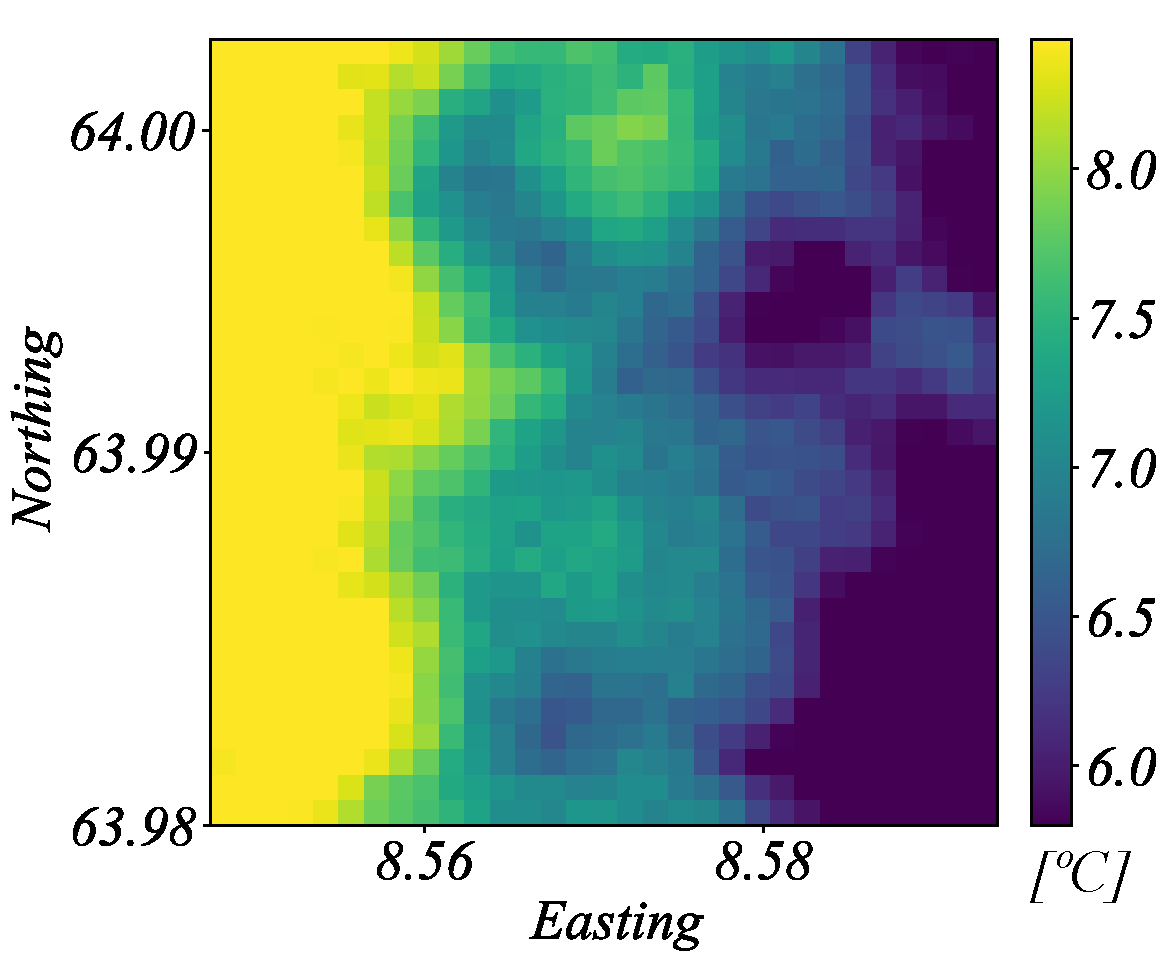
\includegraphics[height = 0.41\textwidth]{Figures/sim/true_temp.pdf}\label{fig:true_temp}}
  \hfill
  \subfigure[Simulated salinity.]{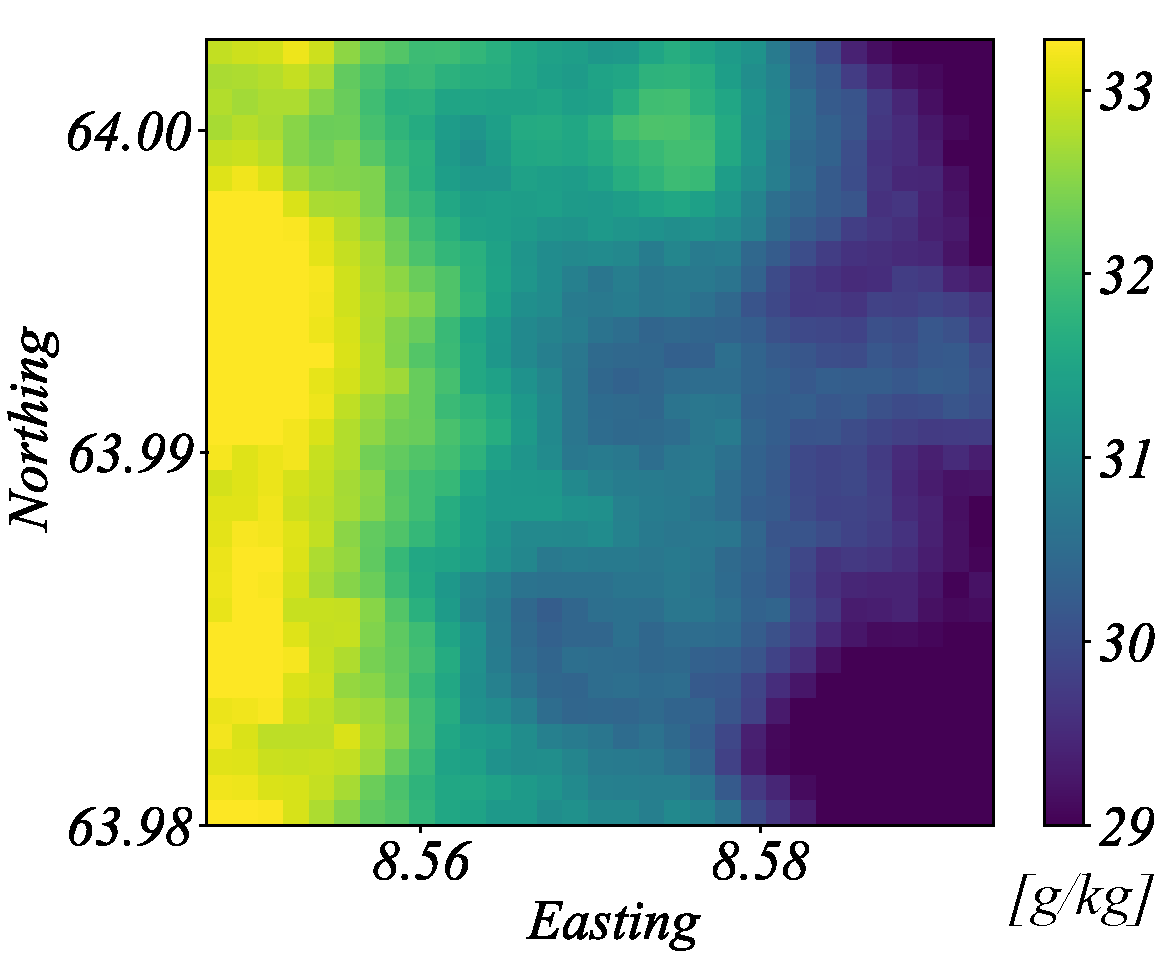
\includegraphics[height = 0.41\textwidth]{Figures/sim/true_sal.pdf}\label{fig:true_sal}}
  \hfill
  \subfigure[Excursion set given the realization of temperature and salinity.]{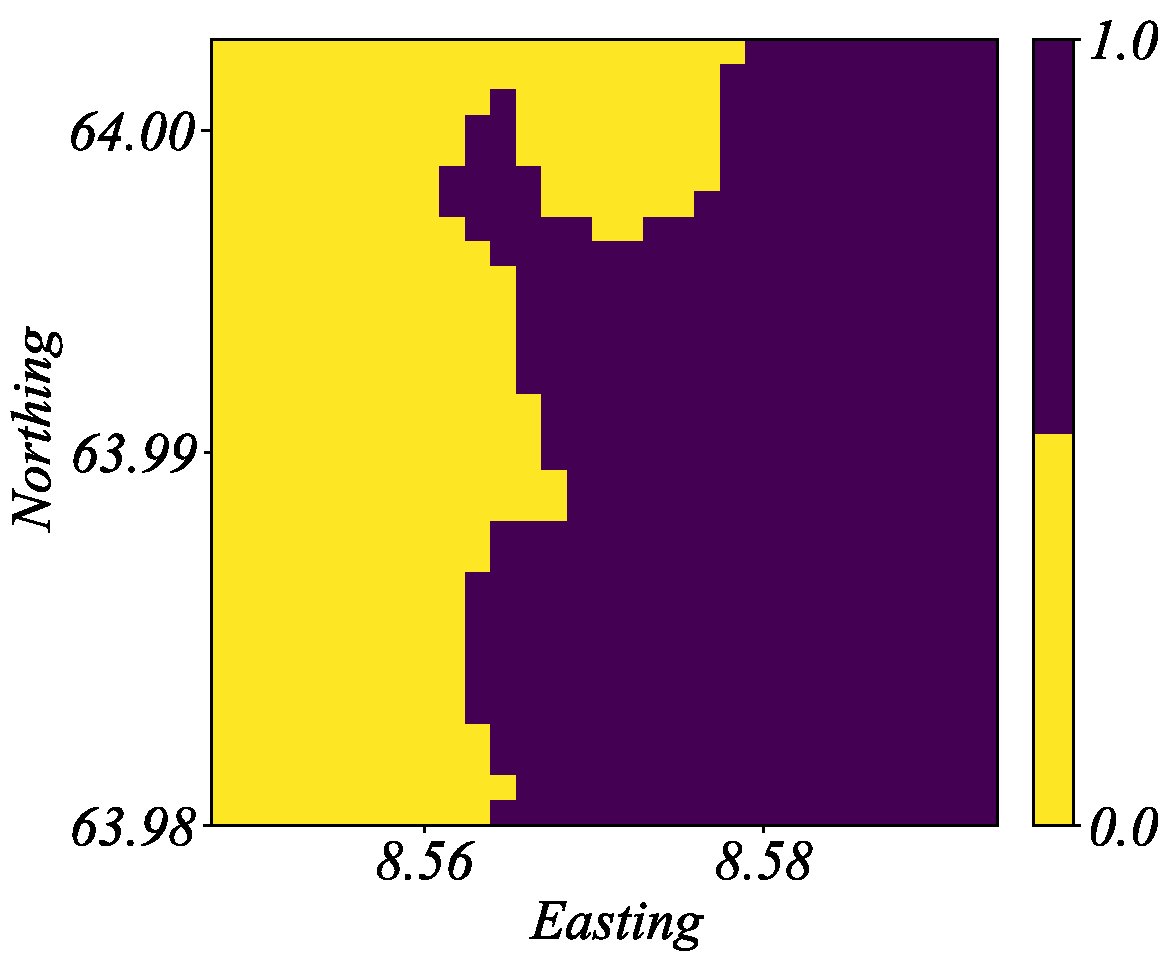
\includegraphics[height = 0.41\textwidth]{Figures/sim/es_ts_true.pdf}\label{fig:ESet}}
  \hfill
  \subfigure[Excursion probabilities given collected data along the strategy ``static\_north".]{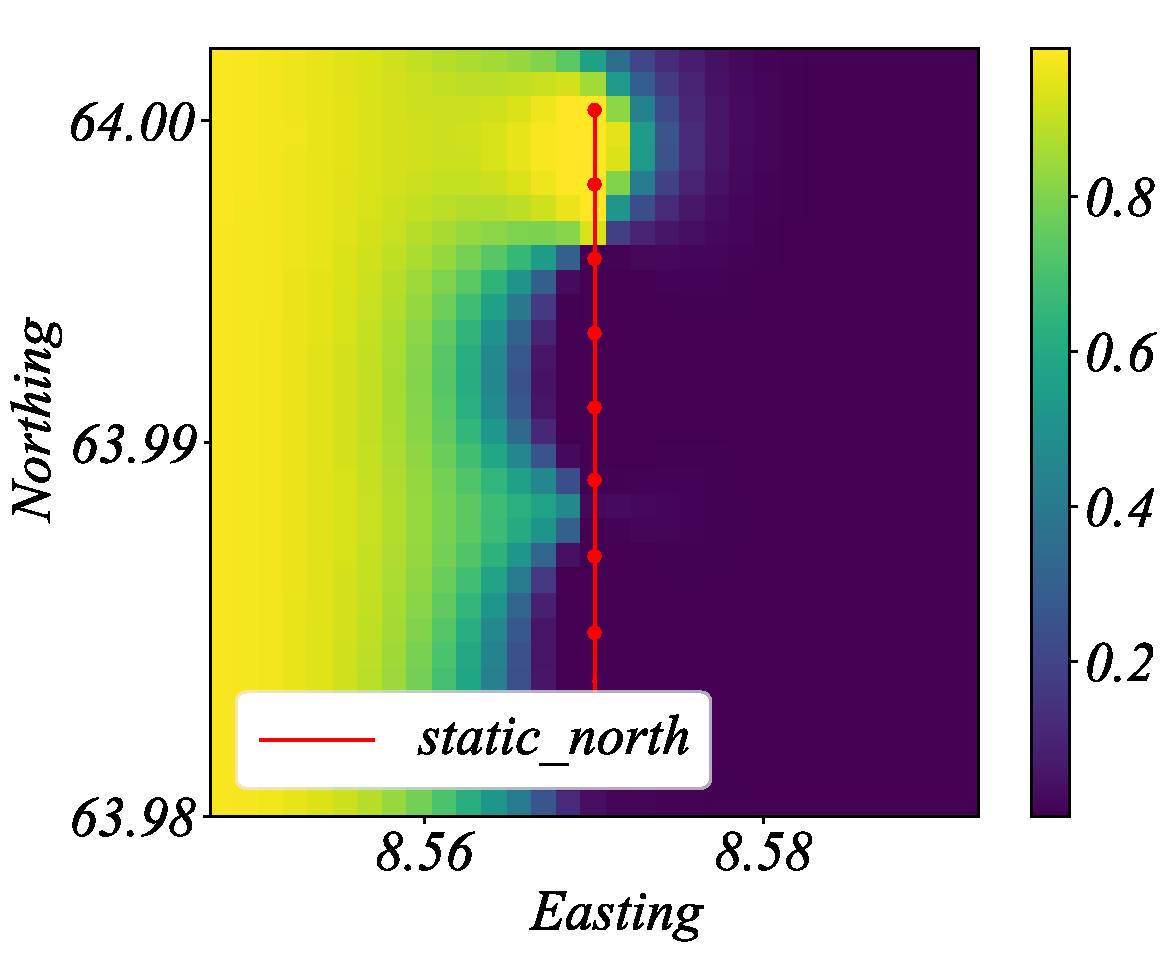
\includegraphics[height = 0.41\textwidth]{Figures/sim/es_ts_posterior.pdf}\label{fig:Eprob}}
  \caption{(\ref{fig:true_temp}) and (\ref{fig:true_sal}) shows
    realisations of the simulated temperature and salinity fields, as
    well as the associated excursion set (\ref{fig:ESet}).
    (\ref{fig:Eprob}) show the estimated excursion probabilities after
    performing data collection along the N-S survey line.} 
\label{fig:realisations}
\end{figure}

The true ES from this prior realization is plotted in Figure \ref{fig:ESet}.
%while the EP ({\bf{what information is this based on? Skip EP here? only ES true? }} )

\subsection{Static and sequential sampling designs}

%Three different designs are considered as indicated in Figure \ref{fig:stat_design}. 
%\begin{figure}[h!]
%\centering
%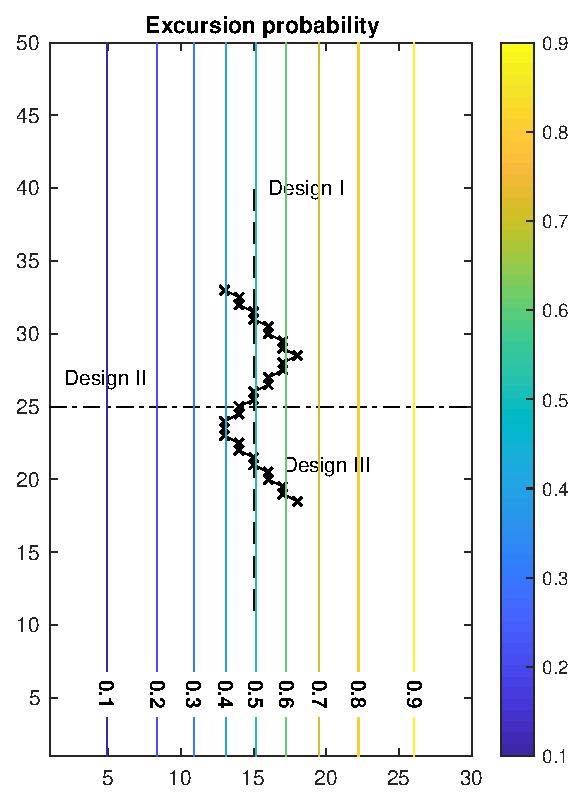
\includegraphics[width=0.65\textwidth]{Figures/Des3.eps}
%\caption{Three different static survey designs plotted on the initial EP.}\label{fig:stat_design}
%\end{figure}
%In this display the designs are plotted along with the prior probability contours of the ES for the reference parameter inputs. 

We compare three different static designs denoted \texttt{static\_north}, \texttt{static\_east and} \texttt{static\_zigzag} with the three sequential approaches \texttt{naive}, \texttt{myopic} and \texttt{look-ahead}. The static sampling paths are pre-determined, and cannot adapt to data. 

For a fixed length, the expected variance after static surveying is analytically available, but here we focus on the properties of the sequential designs which are evaluated using Monte Carlo sampling over several replicates of realizations from the prior, and conducting simulated sequential surveying for each one. For comparison, the same setup is used for the static designs. Figure \ref{fig:Eprob} shows the conditional EP, given data gathered along the north-south survey line for the realization indicated in these displays. In the Monte Carlo replicates, such results are repeatedly computed to approximate the expected variance reduction in the ES. Along with this criterion we also compare predictive performance measured by root mean square error (RMSE) in the temperature and salinity fields and variance reduction in these two field variables. Note that objective function used by the agents is focused on reducing the expected variance in the ES, but we nevertheless hope to achieve good predictive performance for the other criteria as well. Another non-statistical criteria that is important for practical purposes is the computing time of the strategy. 

The agent of the sequential designs starts at the center East-West coordinate at the southern end of the domain (node 53), see Fig. \ref{fig:wp_graph}.

\begin{figure}[h]
\centering
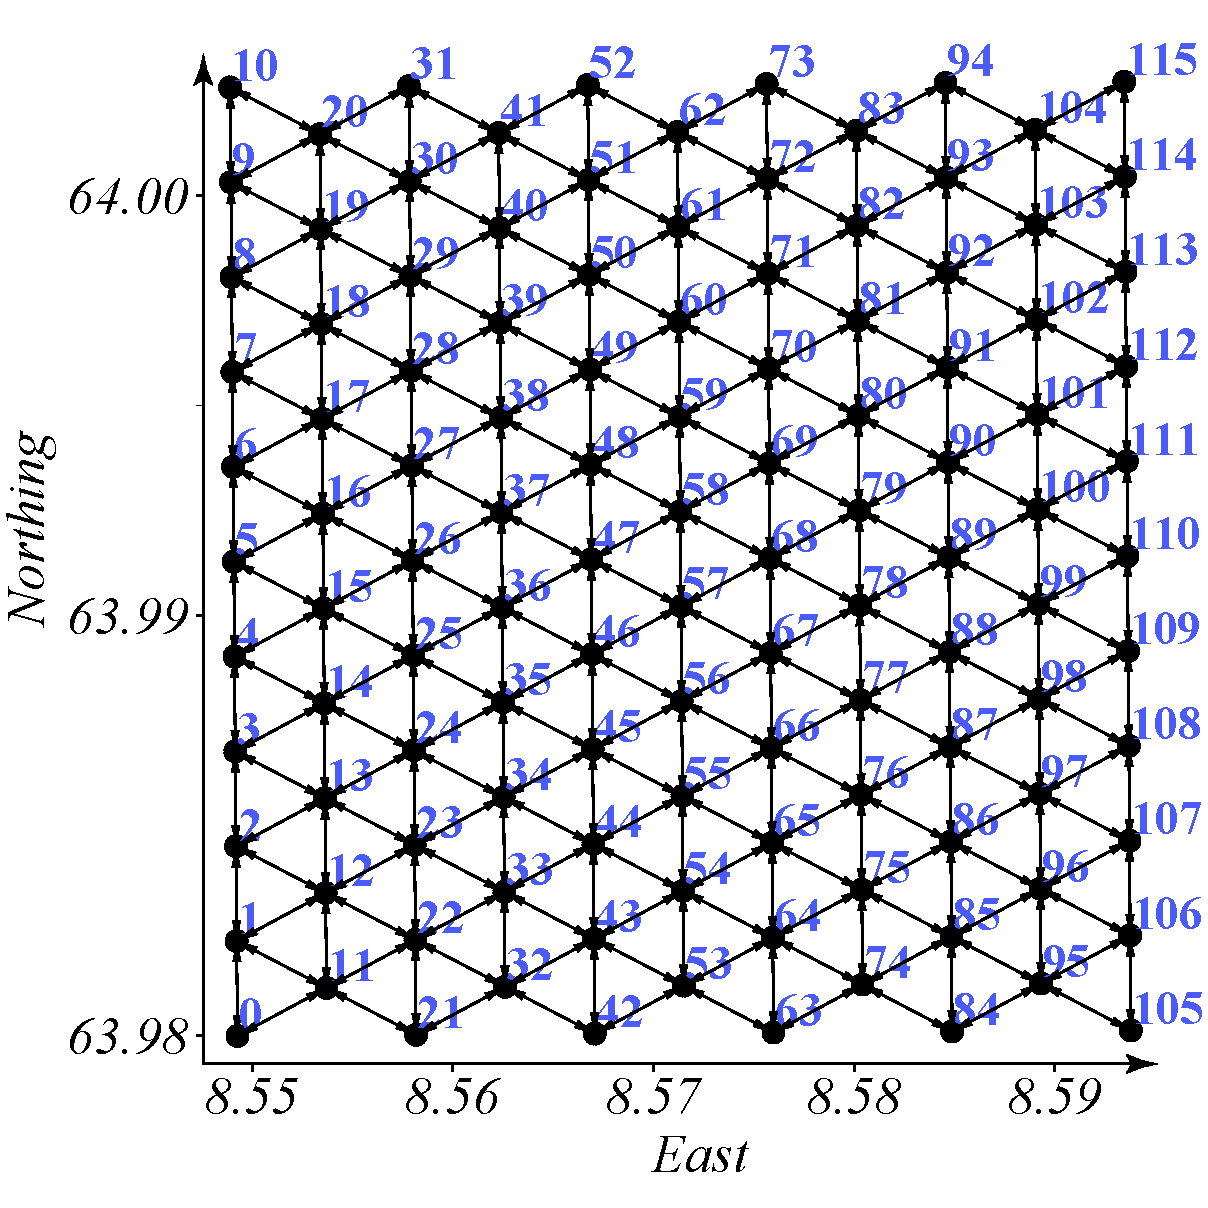
\includegraphics[width=0.50\textwidth]{Figures/sim/wp_graph_paper.pdf}
\caption{The equilateral waypoint graph used to discretize the route choices over the $31\times31$ grid.}
\label{fig:wp_graph}
\end{figure}

At each step, the AUV will choose to move along an edge in this waypoint
graph. While doing so, it gathers three measurements. These are
assimilated in the model, and then a new choice is done at the end of
the edge. The paths of will differ for the various sequential designs.
The designs will also differ between the runs, because the measurements
vary among replicates.


Results of the replicate runs are shown in Figure \ref{fig:sim_results},
where the different criteria are plotted as a function of surveying
distance. Here, expected ES variance in Figure \ref{fig:avg_ev} is
reduced most when using the \texttt{myopic} and \texttt{look-ahead}
strategies. There is not much difference between these two.  


\begin{figure}[!th]
  \centering
  % \subfigure[Excursion set variance $E_y(p[1-p])$.]{\label{fig:avg_ev}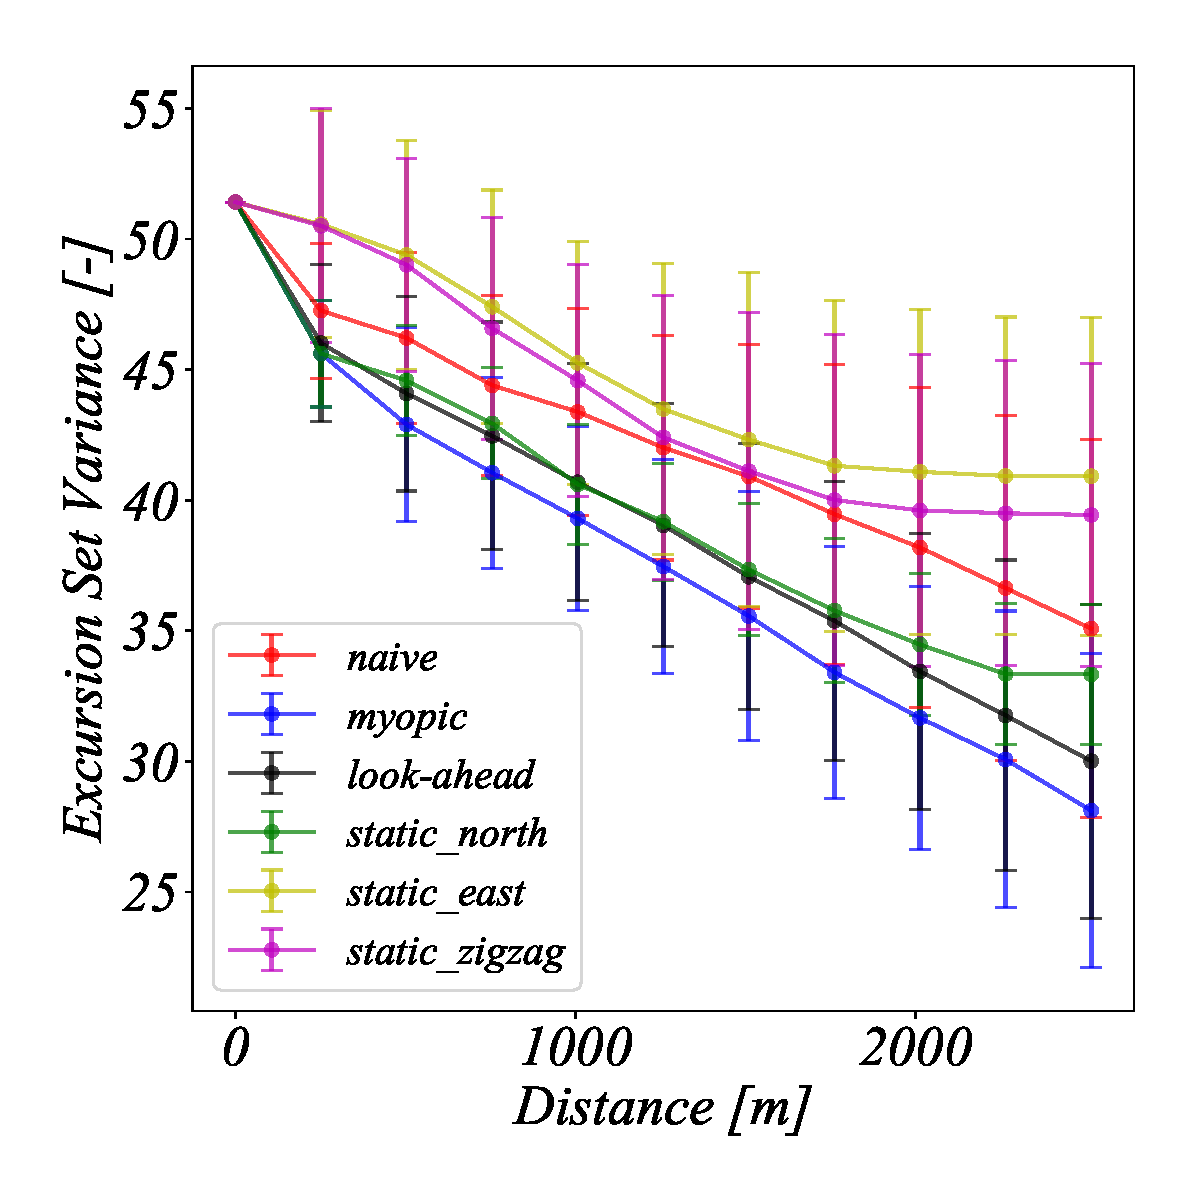
\includegraphics[height=0.49\textwidth]{Figures/sim/avg_EV.pdf}}
  \subfigure[Excursion set $E_y$(p\lbrack 1-p\rbrack) variance.]{\label{fig:avg_ev}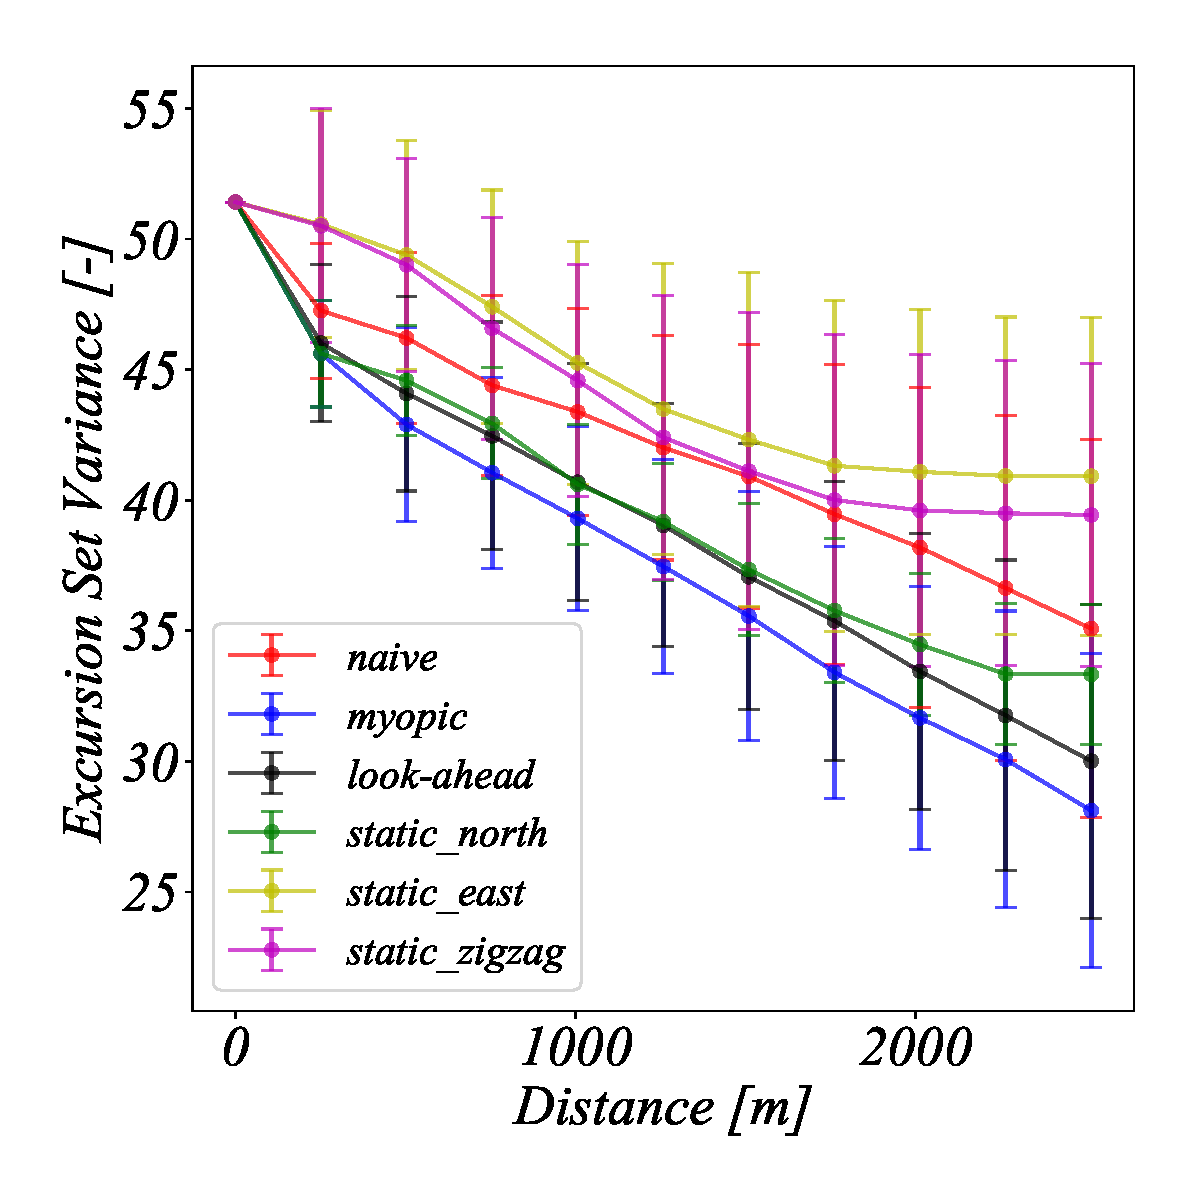
\includegraphics[height=0.49\textwidth]{Figures/sim/avg_EV.pdf}}
  \hfill
  \subfigure[RMSE between estimated field and truth.]{\label{fig:avg_rmse}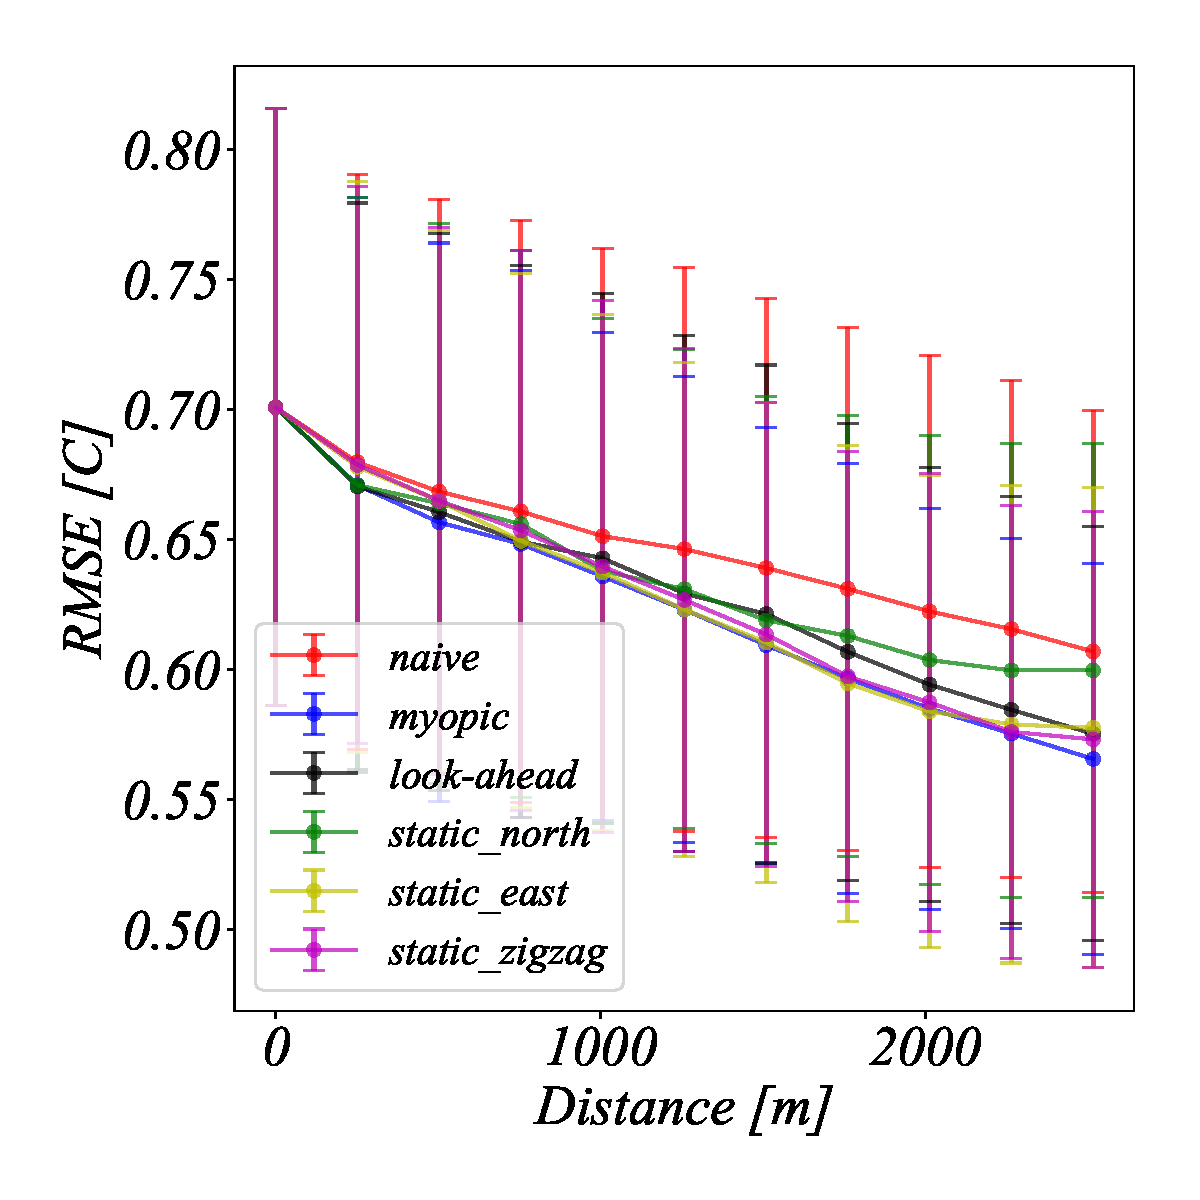
\includegraphics[height=0.49\textwidth]{Figures/sim/avg_RMSE.pdf}}
  \hfill 
  \subfigure[Explained variance $\bR^{2}$.]{\label{fig:avg_r2}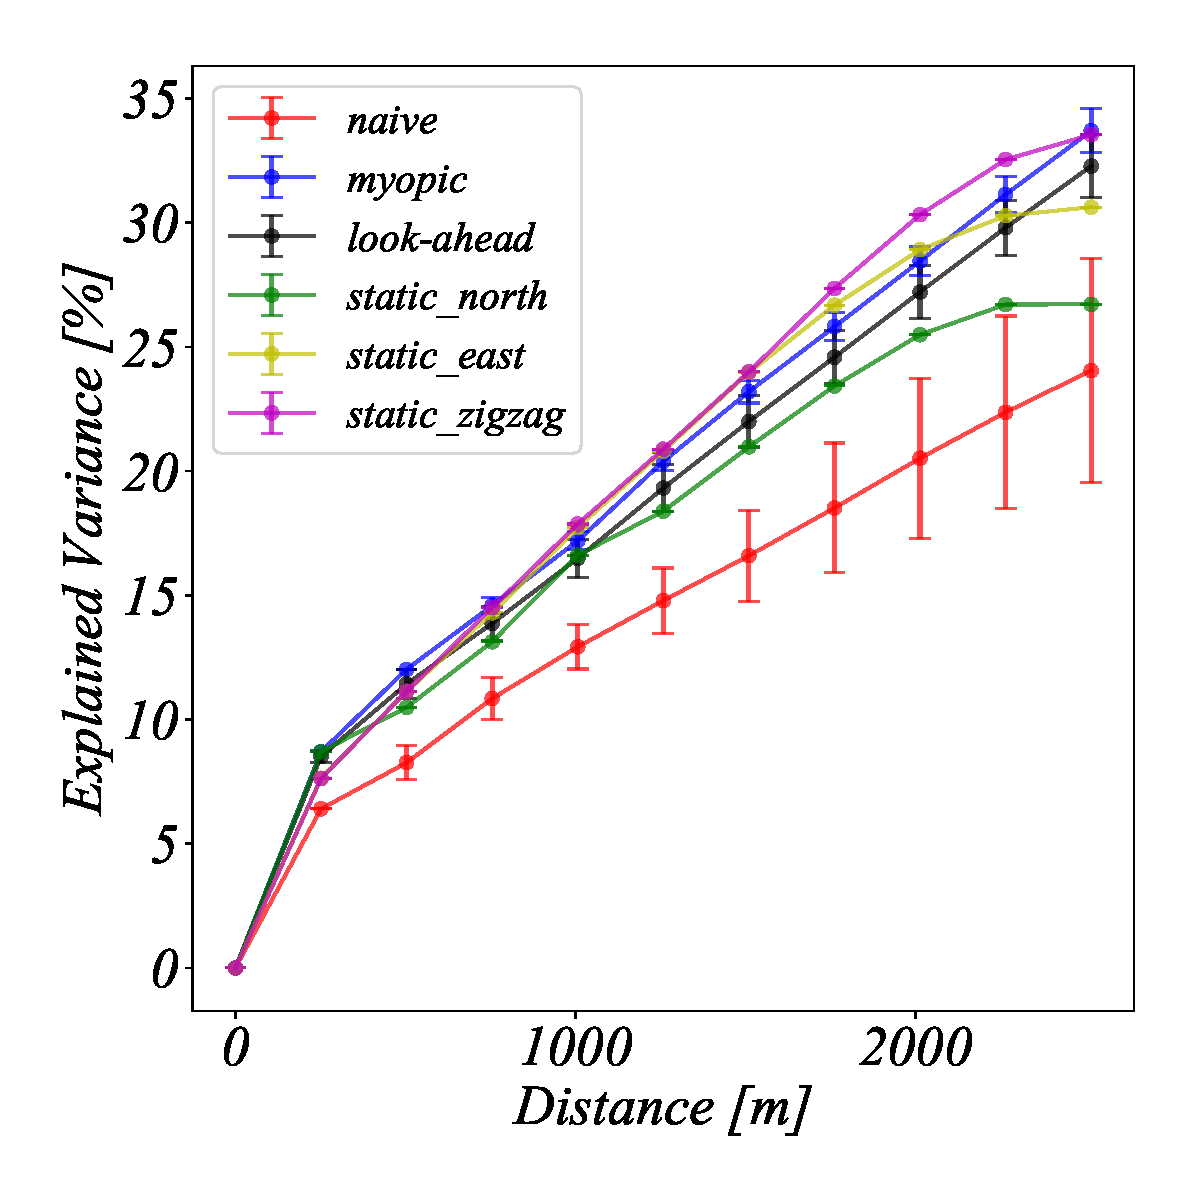
\includegraphics[height=0.49\textwidth]{Figures/sim/avg_R2.pdf}}
  \hfill 
  \subfigure[Time used to do inference.]{\label{fig:avg_time}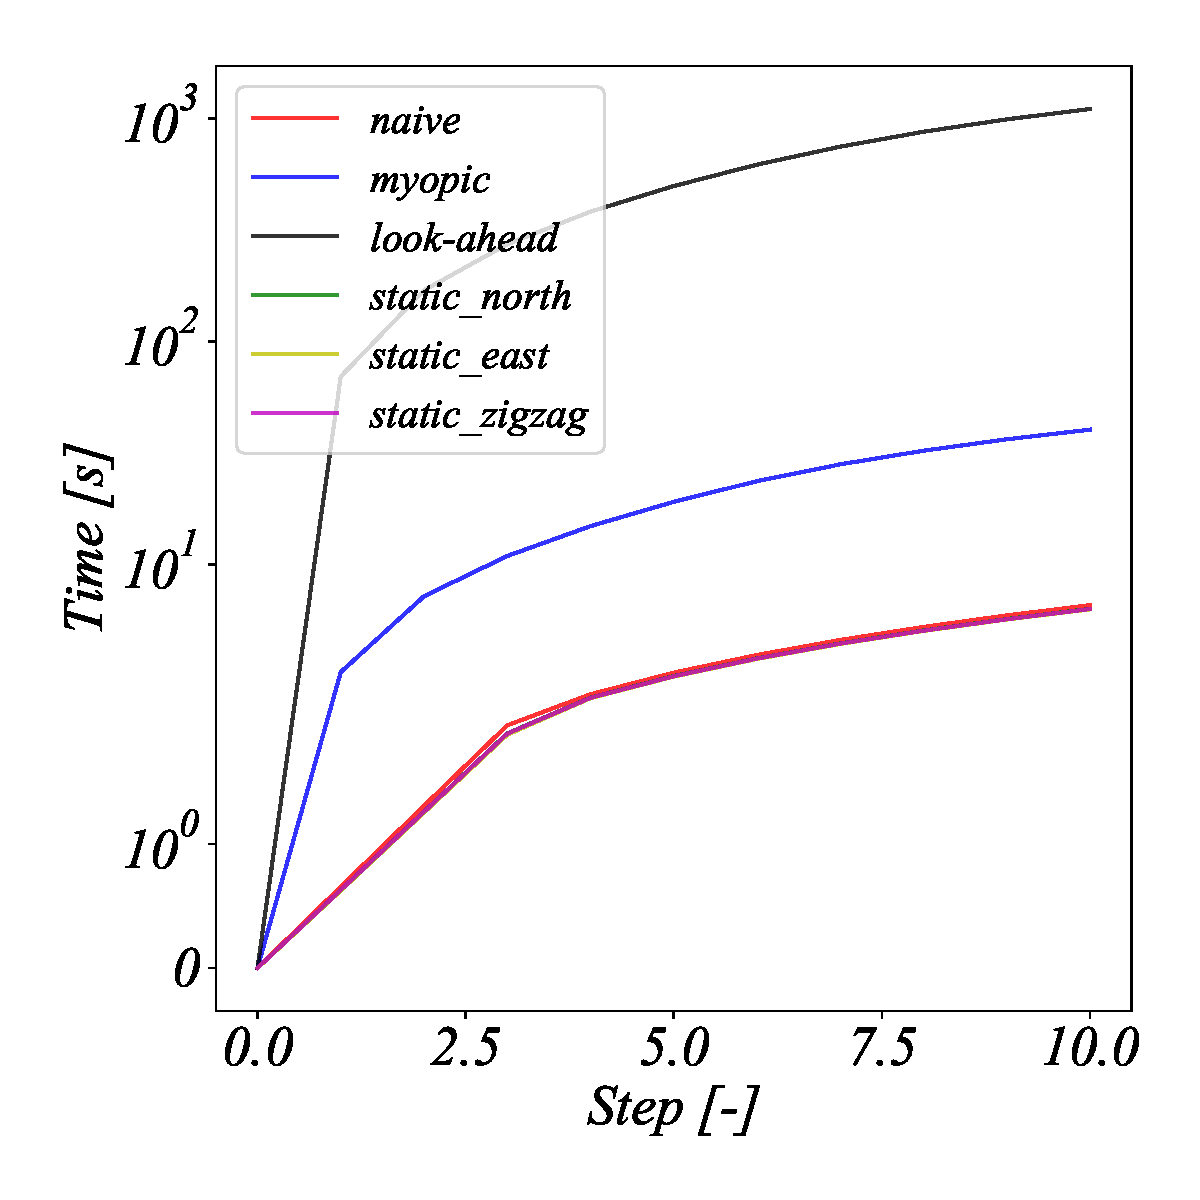
\includegraphics[height=0.49\textwidth]{Figures/sim/avg_Time.pdf}}
\caption{Simulation results from 100 replicate simulations for 10
  sampling choices/steps on the grid. (Updated:01.05.2019)} 
\label{fig:sim_results}
\end{figure}

The north-south design is also doing well, because it moves near the
boundary of the water masses. In Figure \ref{fig:avg_rmse} and
\ref{fig:avg_r2} we show results of RMSE and explained variance. Both
\texttt{myopic} and \texttt{look-ahead} still perform well, but some of
the static east and zigzag are also achieving good results because they
are set to always cover large parts of the domain, and in this way visit
locations that are not considered interesting by the sequential
strategies targeting ES variance. Regarding computing time in Fig.
\ref{fig:avg_time}, the \texttt{naive} strategy is on par with the
static designs, while \texttt{myopic} is slower and \texttt{look-ahead}
much slower. The \texttt{look-ahead} strategy is reaching levels that
are near impractical for on-board execution. Of course, with harder
pruning of branches in the graph, it would be faster to run. Then again,
this pruning is likely the reason that this strategy does not
outperforms the myopic approach.

In Figure \ref{fig:route_choices} we plot the realized sampling paths of
the sequential schemes and static designs.

\begin{figure}[!h]
  \centering
  \subfigure[Look-ahead strategy.]{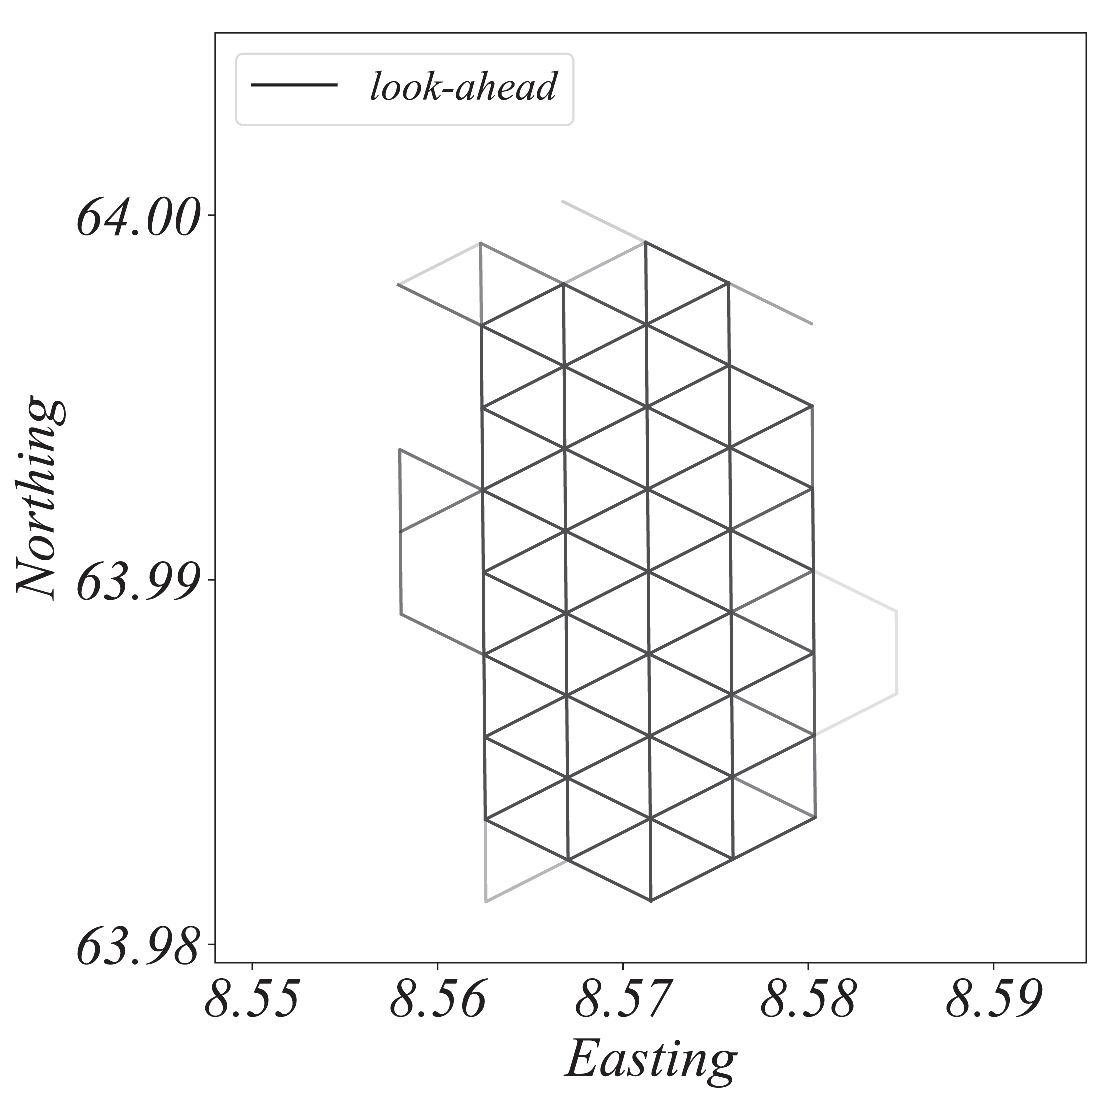
\includegraphics[height = 0.49\textwidth]{Figures/sim/route_look-ahead.pdf}\label{fig:avg_look-ahead}}
  \hfill
  \subfigure[Myopic strategy.]{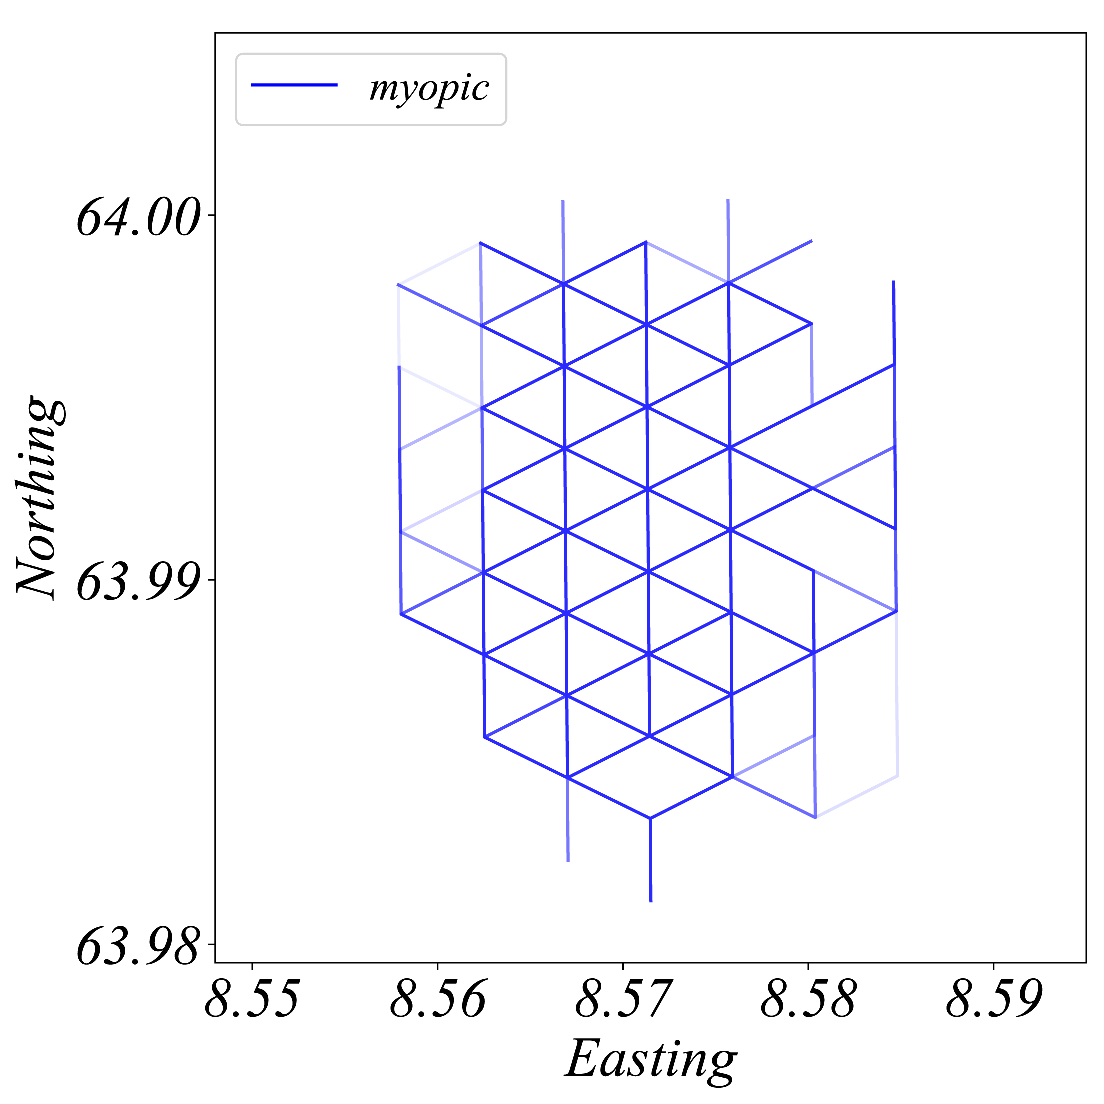
\includegraphics[height = 0.49\textwidth]{Figures/sim/route_myopic.pdf}\label{fig:avg_myopic}}
  \hfill
  \subfigure[Naive strategy.]{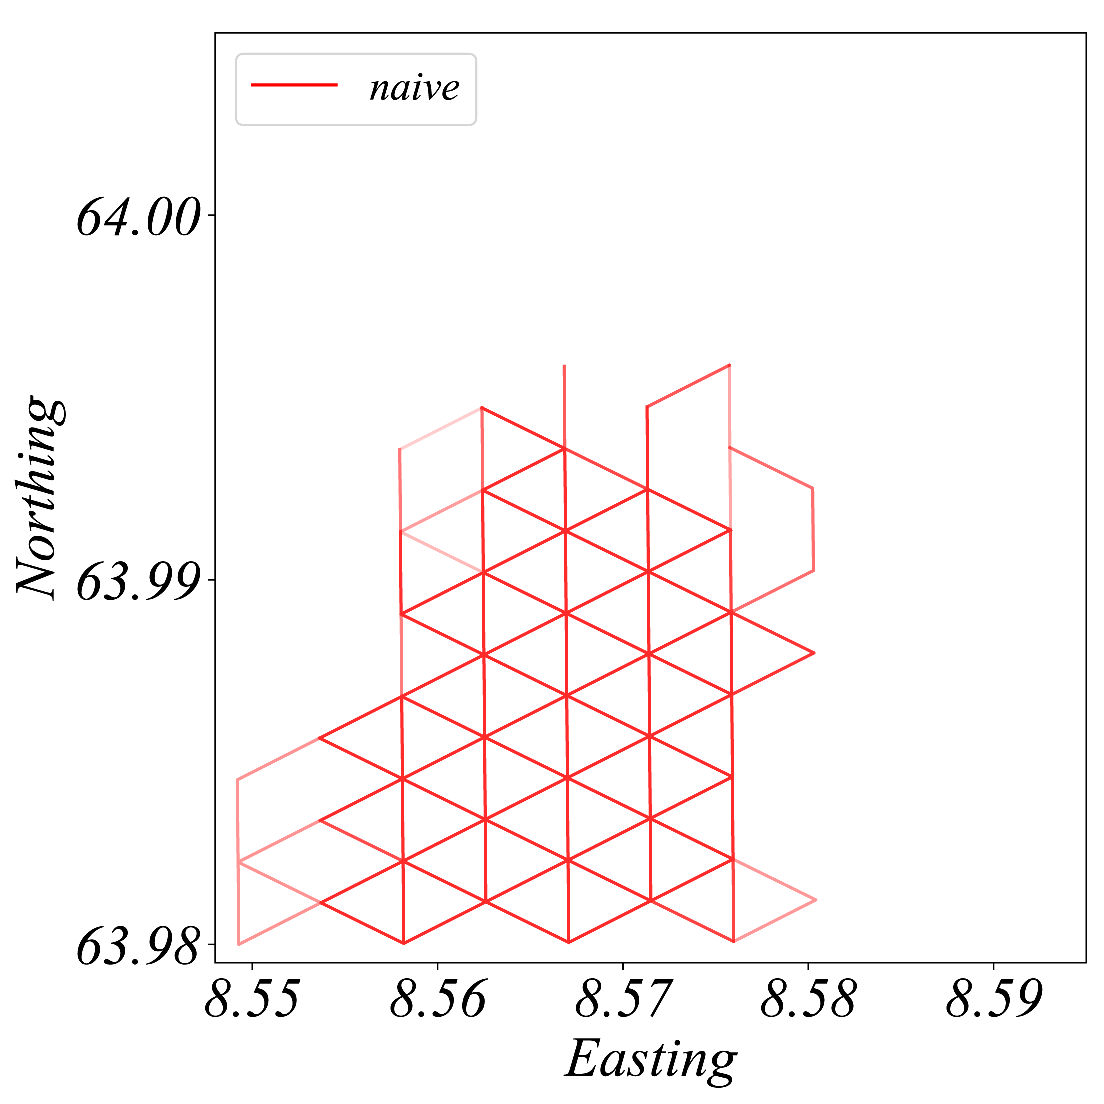
\includegraphics[height = 0.49\textwidth]{Figures/sim/route_naive.pdf}\label{fig:route_naive}}
  \hfill
  \subfigure[Static strategies.]{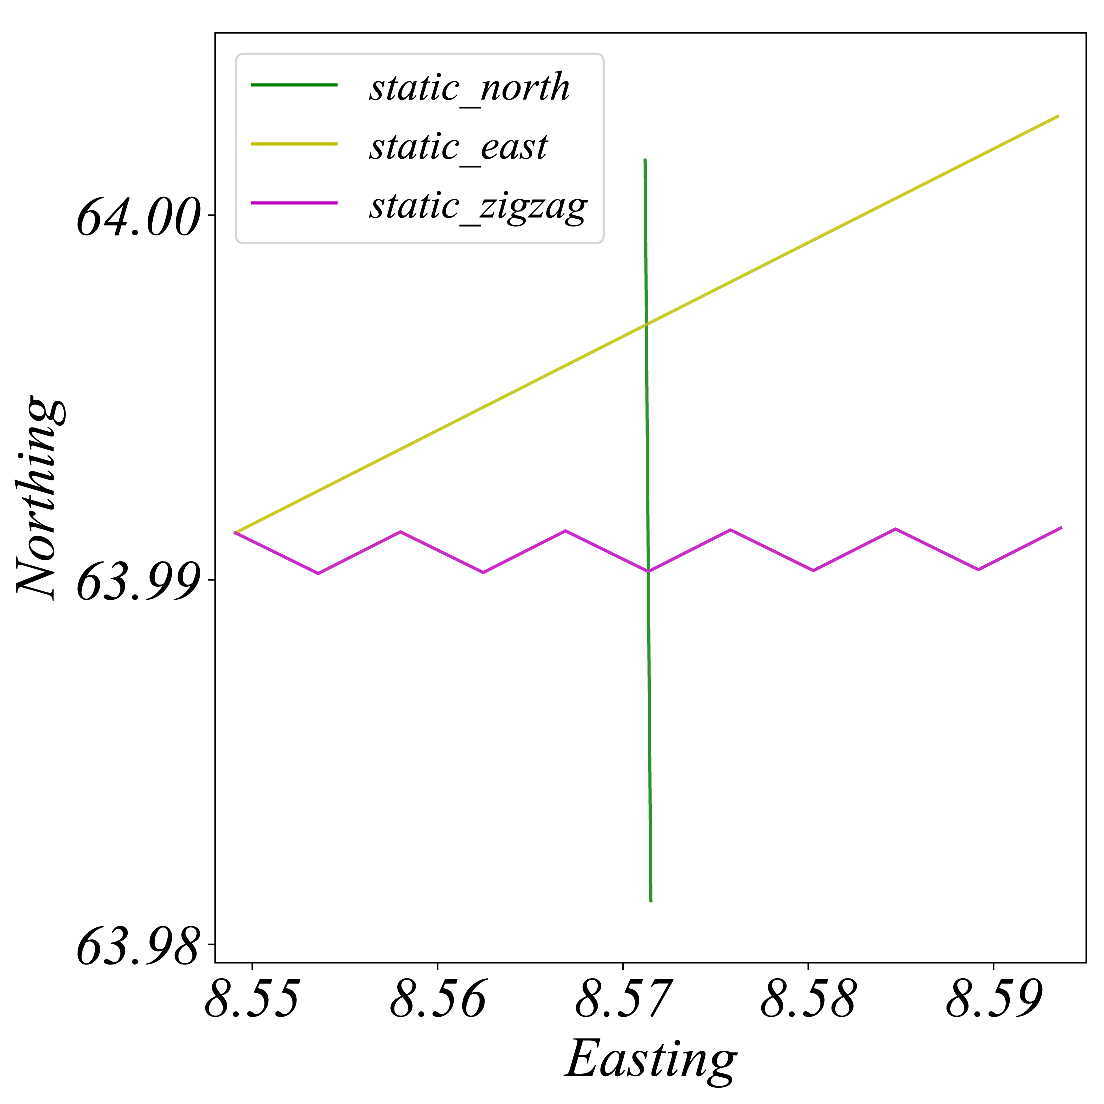
\includegraphics[height = 0.49\textwidth]{Figures/sim/route_static.pdf}\label{fig:route_static}}
  \hfill
\caption{The overlaid route choices, superimposed for the 100 replicate
  surveys with 10 sampling choices/steps.} 
\label{fig:route_choices}
\end{figure}

The naive strategy appears to get stuck in the southern part of the
domain in some cases, because it is too focused on the probabilities
near $0.5$. The myopic strategy seems to be covering a wider domain than
the look-ahead strategy, possibly because the look-ahead strategy sees
less value of going far west because it account for having to return
east again.

We further go on to study sensitivity of the result to different prior correlation values between temperature and salinity, prior standard deviations and spatial correlations, as well as those of measuring only temperature on-board the AUV (as indicated in the rows). We compare results at the end of the surveying distance. Expected ES variances are shown in Table \ref{{tab:sim_res_ev}}. Results of RMSE are in Table \ref{tab:sim_res_rmse} and explained variance in Table \ref{tab:sim_res_r2}. 
In all runs, the myopic and look-ahead strategies perform the best in terms of expected variance in the ES. Surprisingly, the myopic is on-par and even slightly better than the look-ahead strategy. Part of the reason is pruning of paths for the look-ahead strategy, but even with less pruning, the look-ahead does not outperform the myopic approach. Of course, we are able to make up cases where look-ahead beats myopic, but within our ranges of realistic input parameter values it was not easy.
The static north design is clearly better than the other two static designs. The others do not focus on the areas where the ES is really uncertain. 
By measuring temperature alone the expected variances in the ES is only slightly higher. This occurs because the ES is almost the same and because of the correlation of $0.6$ which means that temperature observations give information about salinity as well. 

For the other predictive measures, myopic and look-ahead are still doing well, clearly beating the naive approach. The static zigzag design is usually the best among the static designs for these predictive performance measures because its pattern gives more effective coverage of the domain when there is significant spatial correlation as in this case.
\begin{table}[!h]
    \centering
    \scalebox{0.87}{
    \begin{tabular}{lrrrrrr}
    \toprule
    Parameter: $E_y(p[1-p])$ &  naive &  myopic &  look-ahead &  static\_north &  static\_east &  static\_zigzag \\
    \midrule
                    \rowcolor{Gray}
ts. cor. low: 0.2  &  29.65 &   27.08 &       \textbf{26.44} &         32.33 &        40.31 &          36.23 \\
ts. cor. high: 0.8 &  36.18 &   \textbf{28.42} &       30.30 &         32.99 &        37.18 &          36.04 \\
                    \rowcolor{Gray}
std. low: 0.1      &  18.26 &   15.79 &       \textbf{15.35} &         18.89 &        26.65 &          26.10 \\
std. high: 0.5     &  47.01 &   \textbf{41.31} &       43.15 &         47.92 &        52.63 &          49.71 \\
                    \rowcolor{Gray}
cor. low: 0.8      &  44.42 &   \textbf{42.02} &       42.47 &         43.84 &        46.05 &          47.82 \\
cor. high: 0.2     &  29.73 &   21.09 &       \textbf{20.43} &         27.91 &        37.60 &          34.35 \\
                    \rowcolor{Gray}
temp. only         &  38.25 &   29.16 &       \textbf{28.69} &         34.32 &        39.81 &          36.17 \\
basecase           &  35.21 &   \textbf{28.56} &       28.94 &         33.50 &        39.84 &          39.26 \\
    \bottomrule
    \end{tabular}}
    \caption{Simulation results for the final mean excursion set variance (Eq. \eqref{two_partsK}) for 20 replicates, 8 configurations, and 6 strategies.}
    \label{tab:sim_res_ev}
\end{table}

\begin{table}[!h]
    \centering
    \scalebox{0.92}{
        \begin{tabular}{lrrrrrr}
        \toprule
        Parameter: RMSE &  naive &  myopic &  look-ahead &  static\_north &  static\_east &  static\_zigzag \\
        \midrule
                \rowcolor{Gray}
ts. cor. low: 0.2  &   0.63 &    \textbf{0.57} &        0.59 &          0.62 &         0.57 &           0.59 \\
ts. cor. high: 0.8 &   0.63 &    \textbf{0.59} &        0.61 &          0.64 &         0.60 &           0.60 \\
                \rowcolor{Gray}
std. low: 0.1      &   0.39 &    0.37 &        0.38 &          0.38 &         0.40 &           \textbf{0.35} \\
std. high: 0.5     &   0.85 &    0.82 &        0.84 &          0.82 &         0.83 &           \textbf{0.81} \\  
                \rowcolor{Gray}
cor. low: 0.8      &   0.68 &    0.66 &        0.67 &          0.68 &         0.66 &           \textbf{0.65} \\
cor. high: 0.2     &   0.58 &    0.54 &        0.55 &          0.58 &         0.54 &           \textbf{0.49} \\
                \rowcolor{Gray}
temp. only         &   0.65 &    0.63 &        0.62 &          0.65 &         \textbf{0.61} &           0.62 \\
basecase           &  0.61 &   \textbf{0.56} &       \textbf{0.56} &         0.60 &        0.57 &          0.57 \\
        \bottomrule
        \end{tabular}}
    \caption{Simulation results for the final mean RMSE ($\frac{1}{B} \sum_{b=1}^{B} \sqrt{(\bmu-\tilde{\bmu})^2}$) for 20 replicates, 8 configurations, and 6 strategies.}
    \label{tab:sim_res_rmse}
\end{table}

\begin{table}[!h]
    \centering
    \scalebox{0.95}{
        \begin{tabular}{lrrrrrr}
        \toprule
        Parameter: $\bR^{2}$ &  naive &  myopic &  look-ahead &  static\_north &  static\_east &  static\_zigzag \\
        \midrule
                        \rowcolor{Gray}
ts. cor. low: 0.2  &  27.00 &   33.29 &       32.24 &         26.71 &        30.56 &          \textbf{33.50} \\
ts. cor. high: 0.8 &  23.68 &   \textbf{33.87} &       32.42 &         26.72 &        30.73 &          33.61 \\
                        \rowcolor{Gray}
std. low: 0.1      &  25.38 &   30.80 &       30.29 &         26.09 &        28.75 &          \textbf{31.66} \\
std. high: 0.5     &  26.11 &   34.22 &       32.48 &         26.95 &        31.77 &          \textbf{34.48} \\
                        \rowcolor{Gray}
cor. low: 0.8      &   8.80 &   11.50 &       11.23 &          9.56 &        12.31 &          \textbf{12.58} \\
cor. high: 0.2     &  37.57 &   \textbf{48.68} &       48.11 &         39.61 &        41.98 &          48.04 \\
                        \rowcolor{Gray}
temp. only         &  11.67 &   \textbf{22.82} &       21.98 &         18.16 &        20.77 &          22.78 \\
basecase           &  24.71 &   33.45 &       32.25 &         26.71 &        30.62 &          \textbf{33.54}\\
        \bottomrule
        \end{tabular}}
    \caption{Simulation results for the final mean explained variance ($\bR^{2}=100*(1-(\bSigma_{posterior}/\bSigma_{initial}))$) for 20 replicates, 8 configurations, and 6 strategies.}
    \label{tab:sim_res_r2}
\end{table}

\section{Case study}\label{sec:case_study}

\begin{itemize}
    \item Tune prior mean, standard deviations and correlation parameters from ocean model simulations and initial runs. 
    \item Run tests 16 May or 21 May.
\end{itemize} 


\newpage

\section{Closing remarks}\label{sec:concl_disc}

Additional flexibility can be gained by having two AUVs exploring together. It might then be useful to sample different parts of the space, and maybe move in parallel to best capture the excursion set. 

\section*{Acknowledgements}
Thanks to SINTEF Ocean, AMOS, etc..

%\begin{supplement}
%\sname{Supplement A}\label{suppA}
%\stitle{Title of the Supplement A}
%\slink[url]{http://www.e-publications.org/ims/support/dowload/imsart-ims.zip}
%\sdescription{Dum esset rex in
%accubitu suo, nardus mea dedit odorem suavitatis. Quoniam confortavit
%seras portarum tuarum, benedixit filiis tuis in te. Qui posuit fines tuos}
%\end{supplement}

% == Adding references
\footnotesize
\bibliographystyle{apalike}
\bibliography{ref}


% AOS,AOAS: If there are supplements please fill:
%\begin{supplement}[id=suppA]
%  \sname{Supplement A}
%  \stitle{Title}
%  \slink[doi]{10.1214/00-AOASXXXXSUPP}
%  \sdatatype{.pdf}" 
%  \sdescription{Some text}
%\end{supplement}


\end{document}

%\begin{enumerate}
%\item  This is the first item of an enumerated list.  Each item
%      in the list is marked with a ``tick.''  The document
%      style determines what kind of tick mark is used.
%\item  This is the second item of the list.  It contains another
%      list nested inside it.  The three inner lists are an {\em enumerated}
%      list.
%    \begin{enumerate}
%       \item This is the first item of an enumerated list that
%            is nested within the enumerated list.
%          \item This is the second item of the inner list.  \LaTeX\
%            allows you to nest lists deeper than you really should.
%      \end{enumerate}
%      This is the rest of the second item of the outer list.  It
%      is no more interesting than any other part of the item.
%   \item  This is the third item of the list.
%\end{enumerate}